\section{1174050 Dika Sukma Pradana}

\subsection{Teori}
\begin{enumerate}
\item Jelaskan Apa Itu binari calssification dilengkapi ilustrasi gambar sendiri.\par
Klasifikasi biner atau binomial adalah tugas untuk mengklasifikasikan elemen-elemen dari himpunan tertentu ke dalam dua kelompok (memprediksi kelompok mana yang masing-masing dimiliki) berdasarkan aturan klasifikasi.
\begin{figure}[ht]
\centering
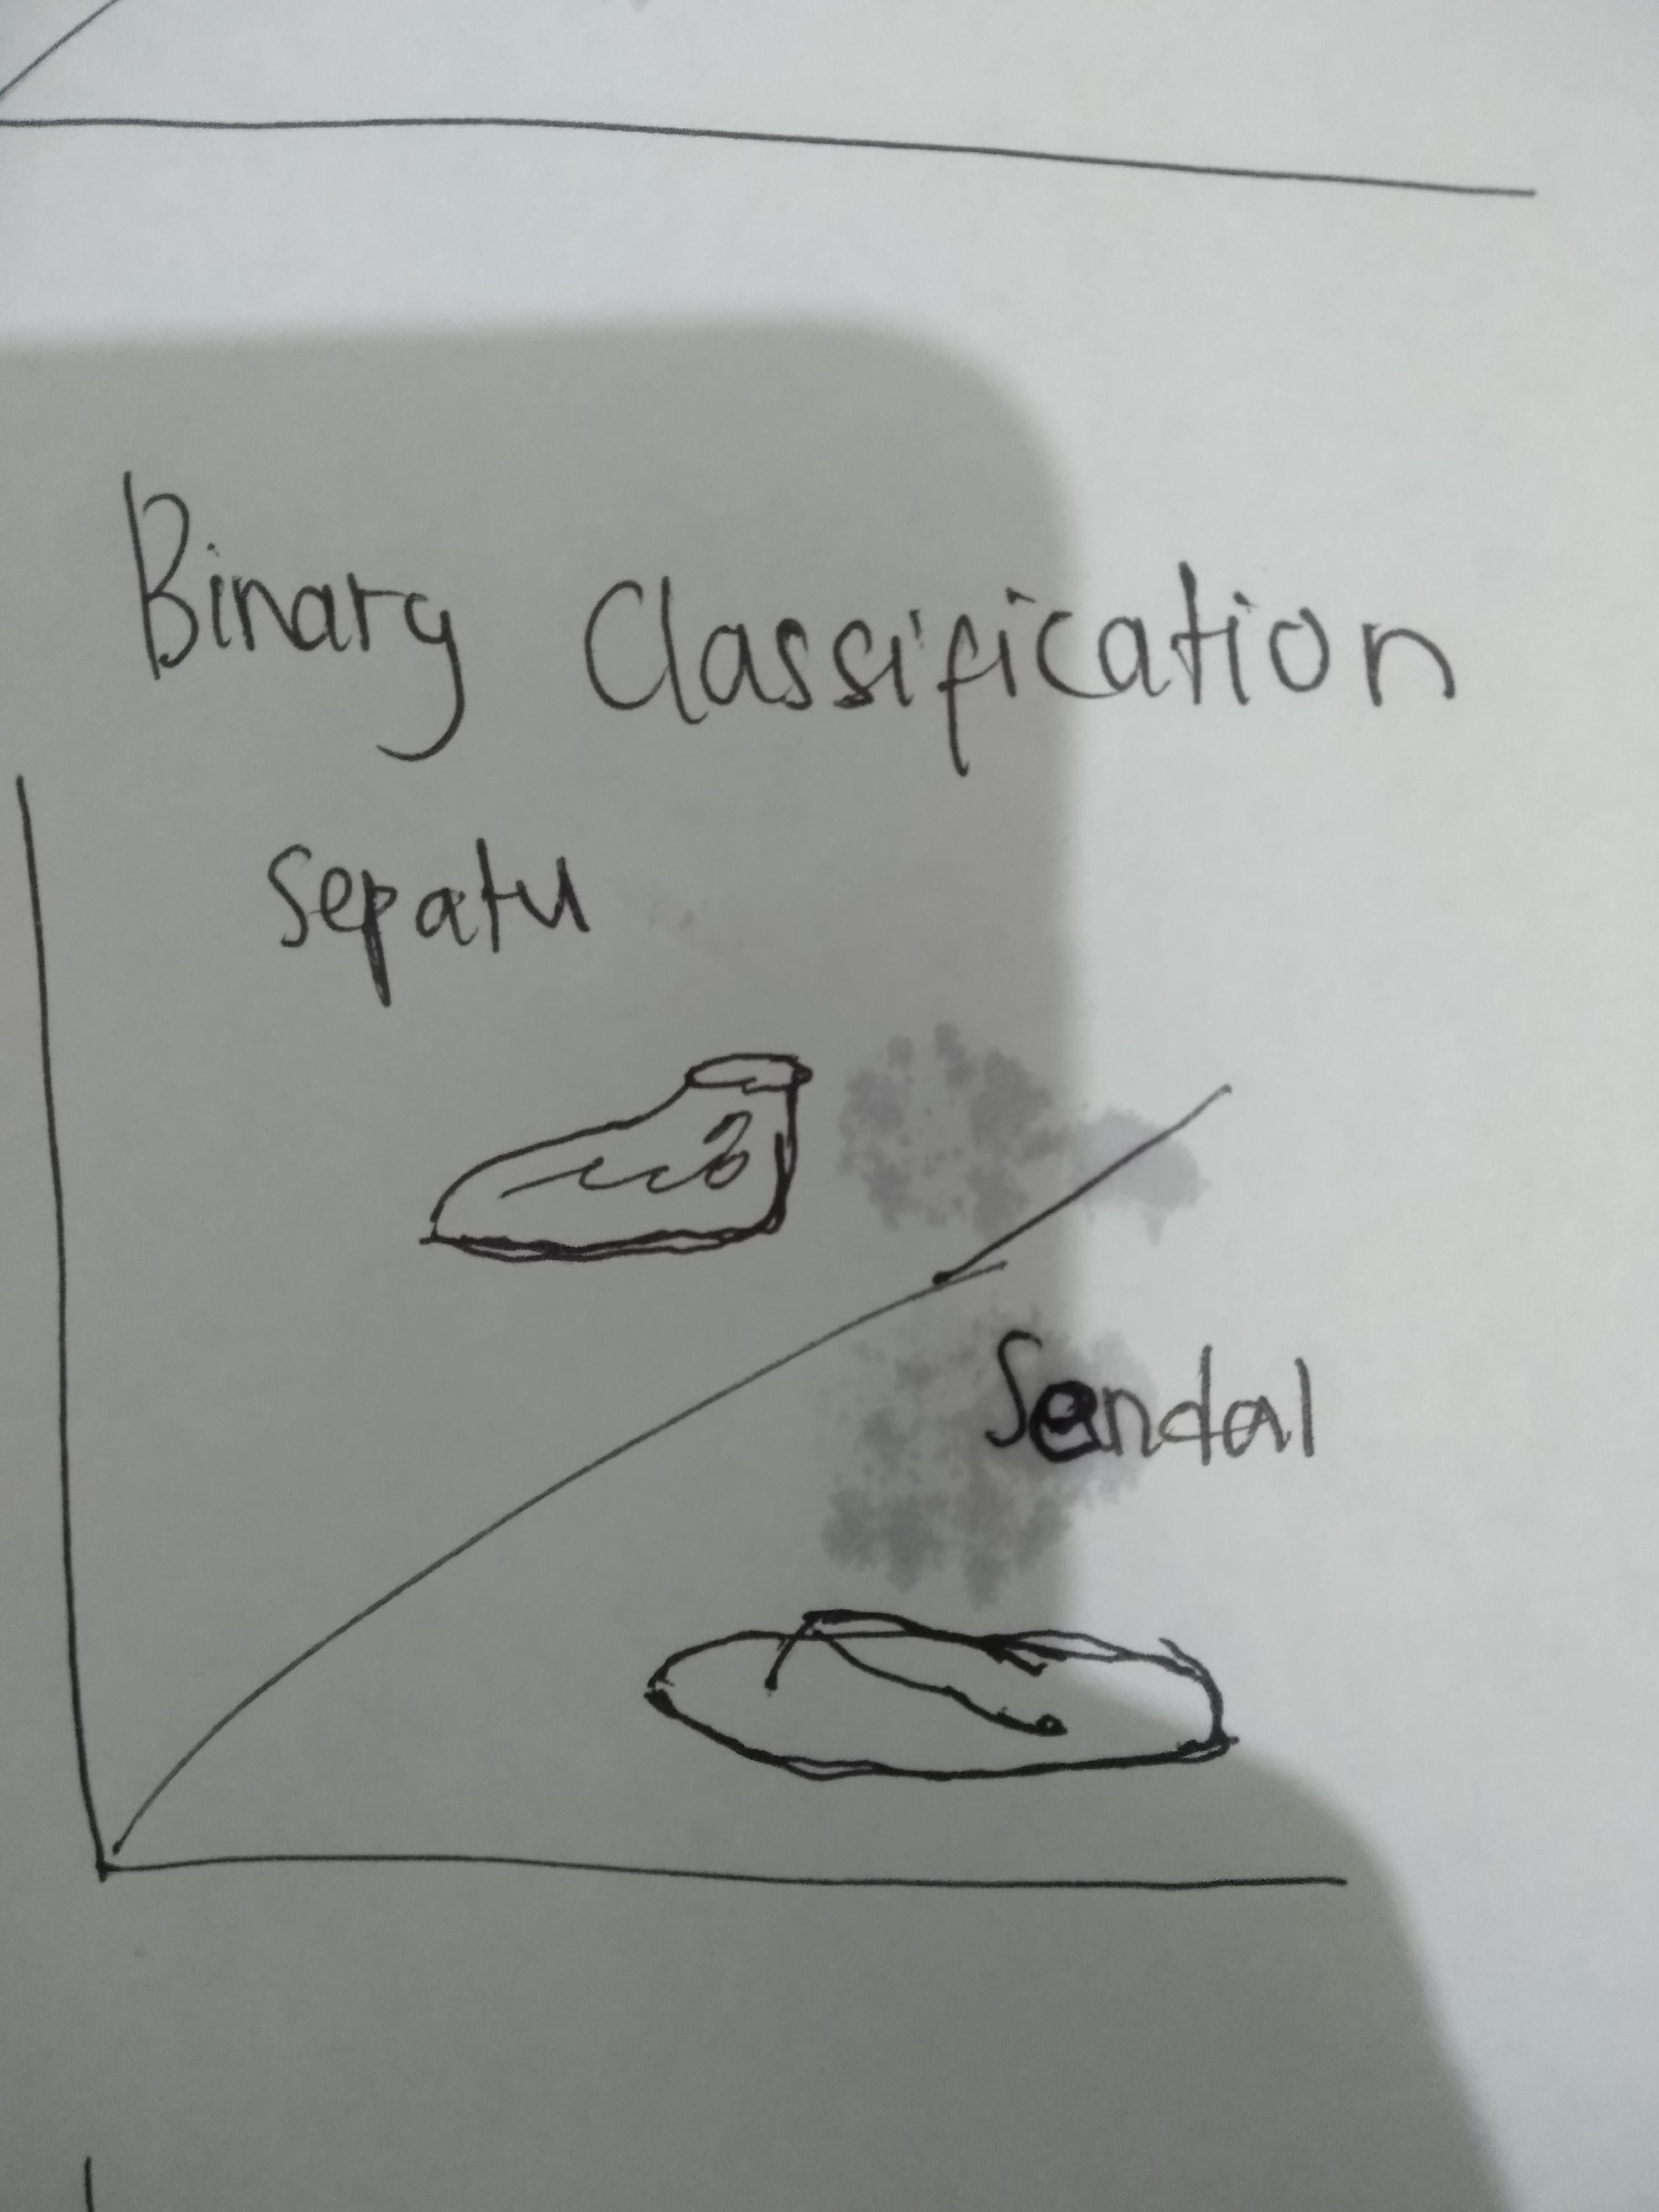
\includegraphics[scale=0.01]{figures/1174050/chapter2/1.jpg}
\caption{contoh binari calssification}
\label{contoh}
\end{figure}


\item Jelaskan Apaitu supervised learning , unsupervised learning dan clusterring dengan ilustrasi gambar sendiri.\par
sSupervised learning adalah sebuah metode pendekatan yang mana sudah terdapat data yang dilatiih, dan terdapat variabel yang ditargetkan atau yang menjadi tujuan sehingga tujuan dari pendekatan ini adalah mengkelompokan suatu data ke data yang sudah ada.  contoh pada nasi termasuk yang mengandung karbohidrat berarti nasi telah di kategorikan kedalam karbohidrat. sedangkan ayam mengandung protein yang berarti ayam telah di kategorikan  yang mengandung protein untuk lebih jelasnya dapat dilihat pada gambar.\par
\begin{figure}[ht]
\centering
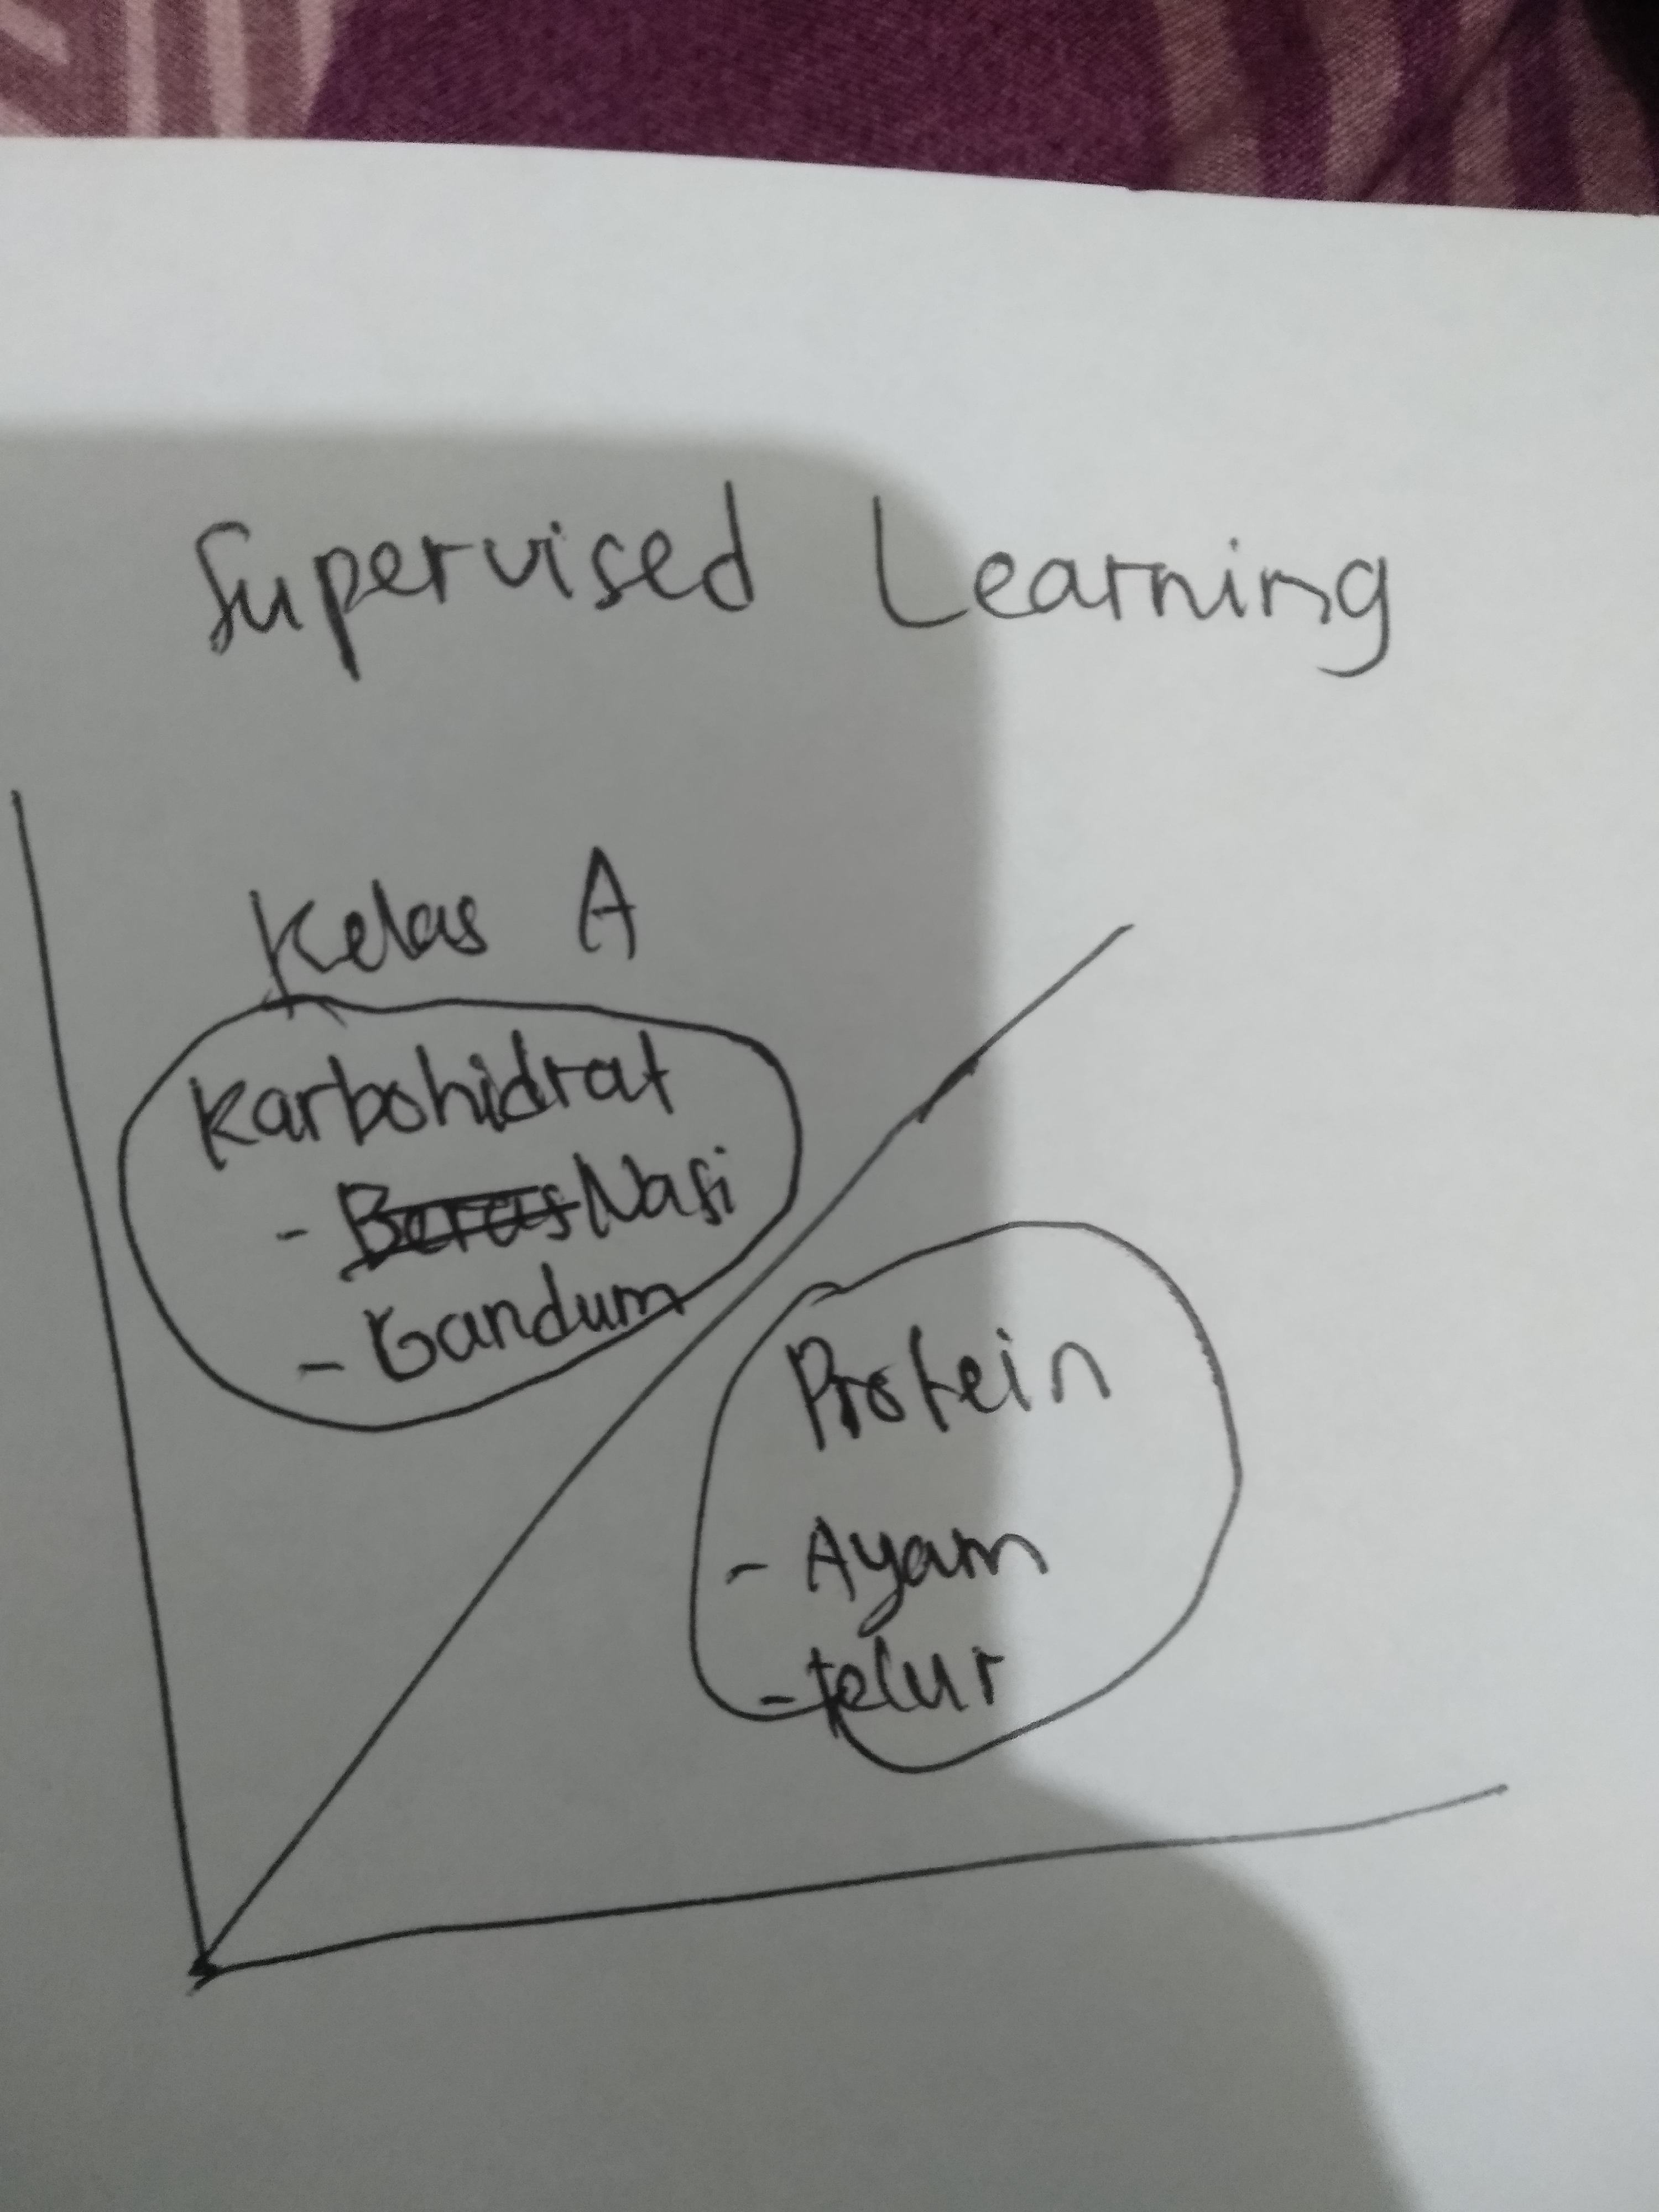
\includegraphics[scale=0.01]{figures/1174050/chapter2/2.jpg}
\caption{contoh supervised learning}
\label{contoh}
\end{figure}

Sedangkan unsupervised learrning tidak memiliki data latiih, sehinggga dari data yang ada, kita mengelompokan data tersebbut menjadi dua bagian atau bahkan tiga bagian dan seterusnya.contoh ayam di kategorikan kedalam karbohidrat untuk lebih jelasnya dapat dilihat pada gambar.\par
\begin{figure}[ht]
\centering
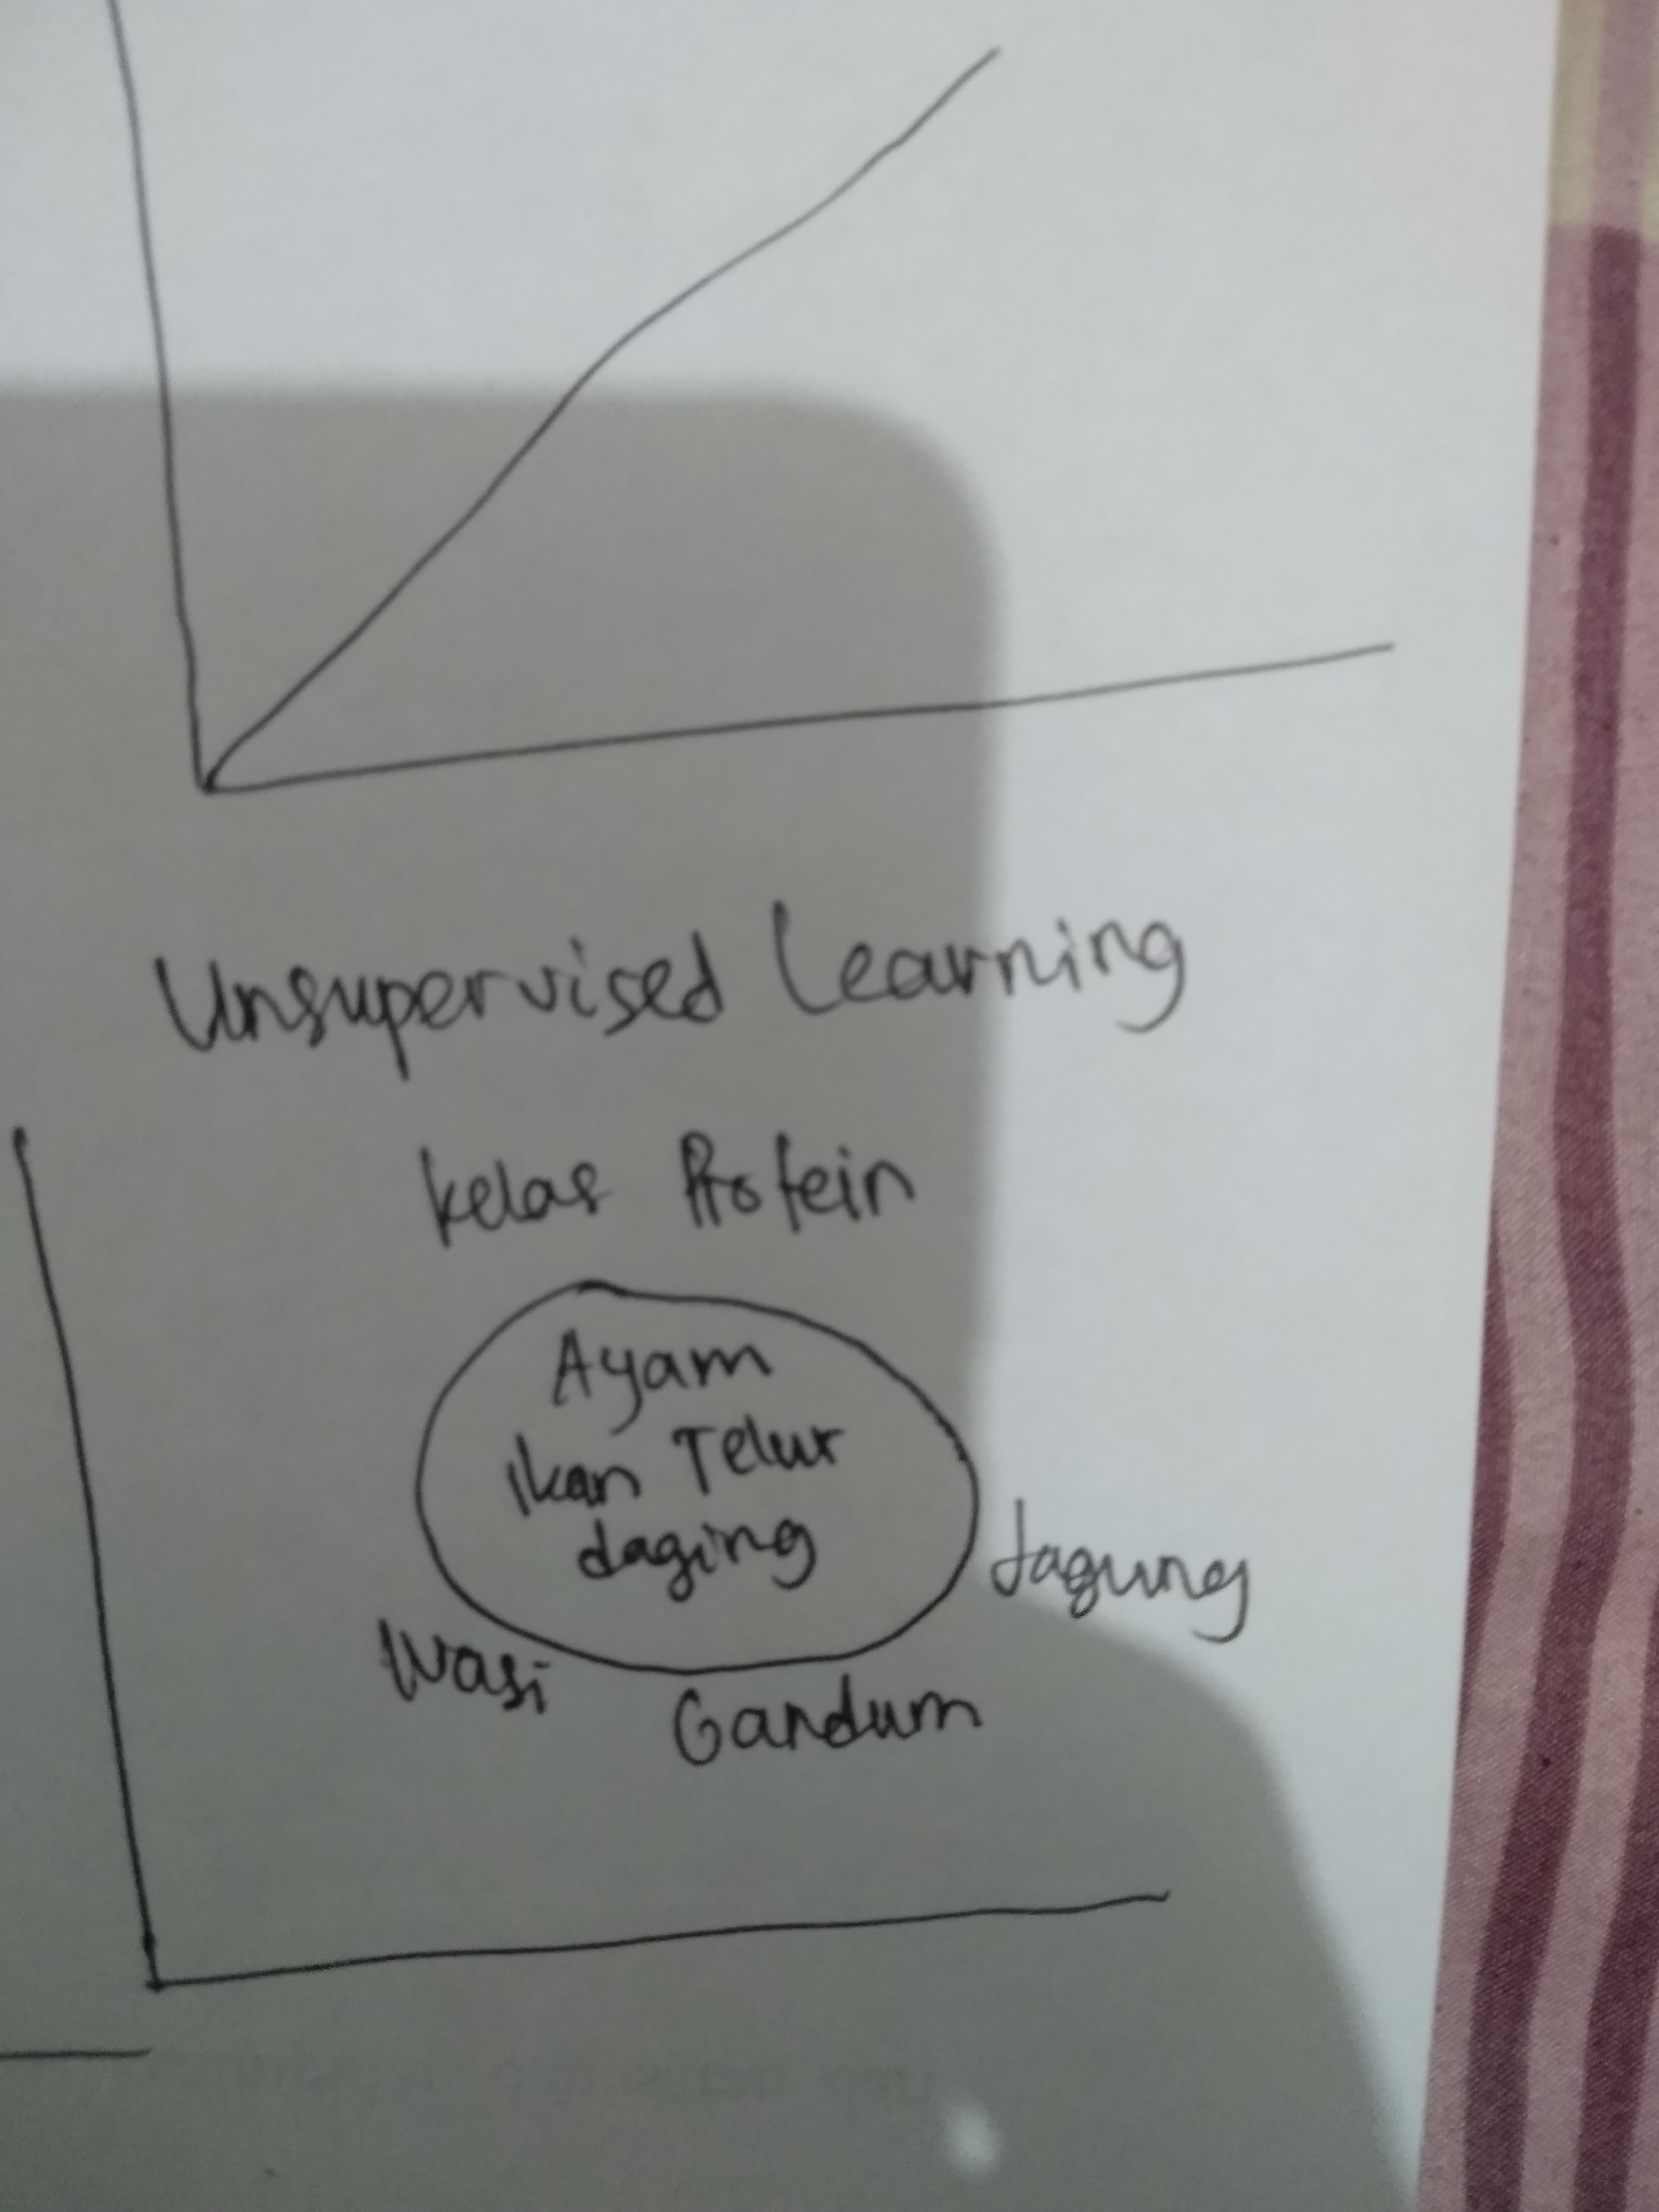
\includegraphics[scale=0.01]{figures/1174050/chapter2/3.jpg}
\caption{contoh unsupervised learning}
\label{contoh}
\end{figure}

clustering merupakan peroses mengklasifikasikan yang berdasarkan suatu parameter dalam penentuannya contoh pada berat protein memiliki berat 1000 gr dan karbohidrat memiliki berat 1200 gr yang berarti berat dibagi dua parameter yaitu lebih kecil samadengan 1000 gram dan lebih besar dari 1000gram contoh pada gambar.\par
\begin{figure}[ht]
\centering
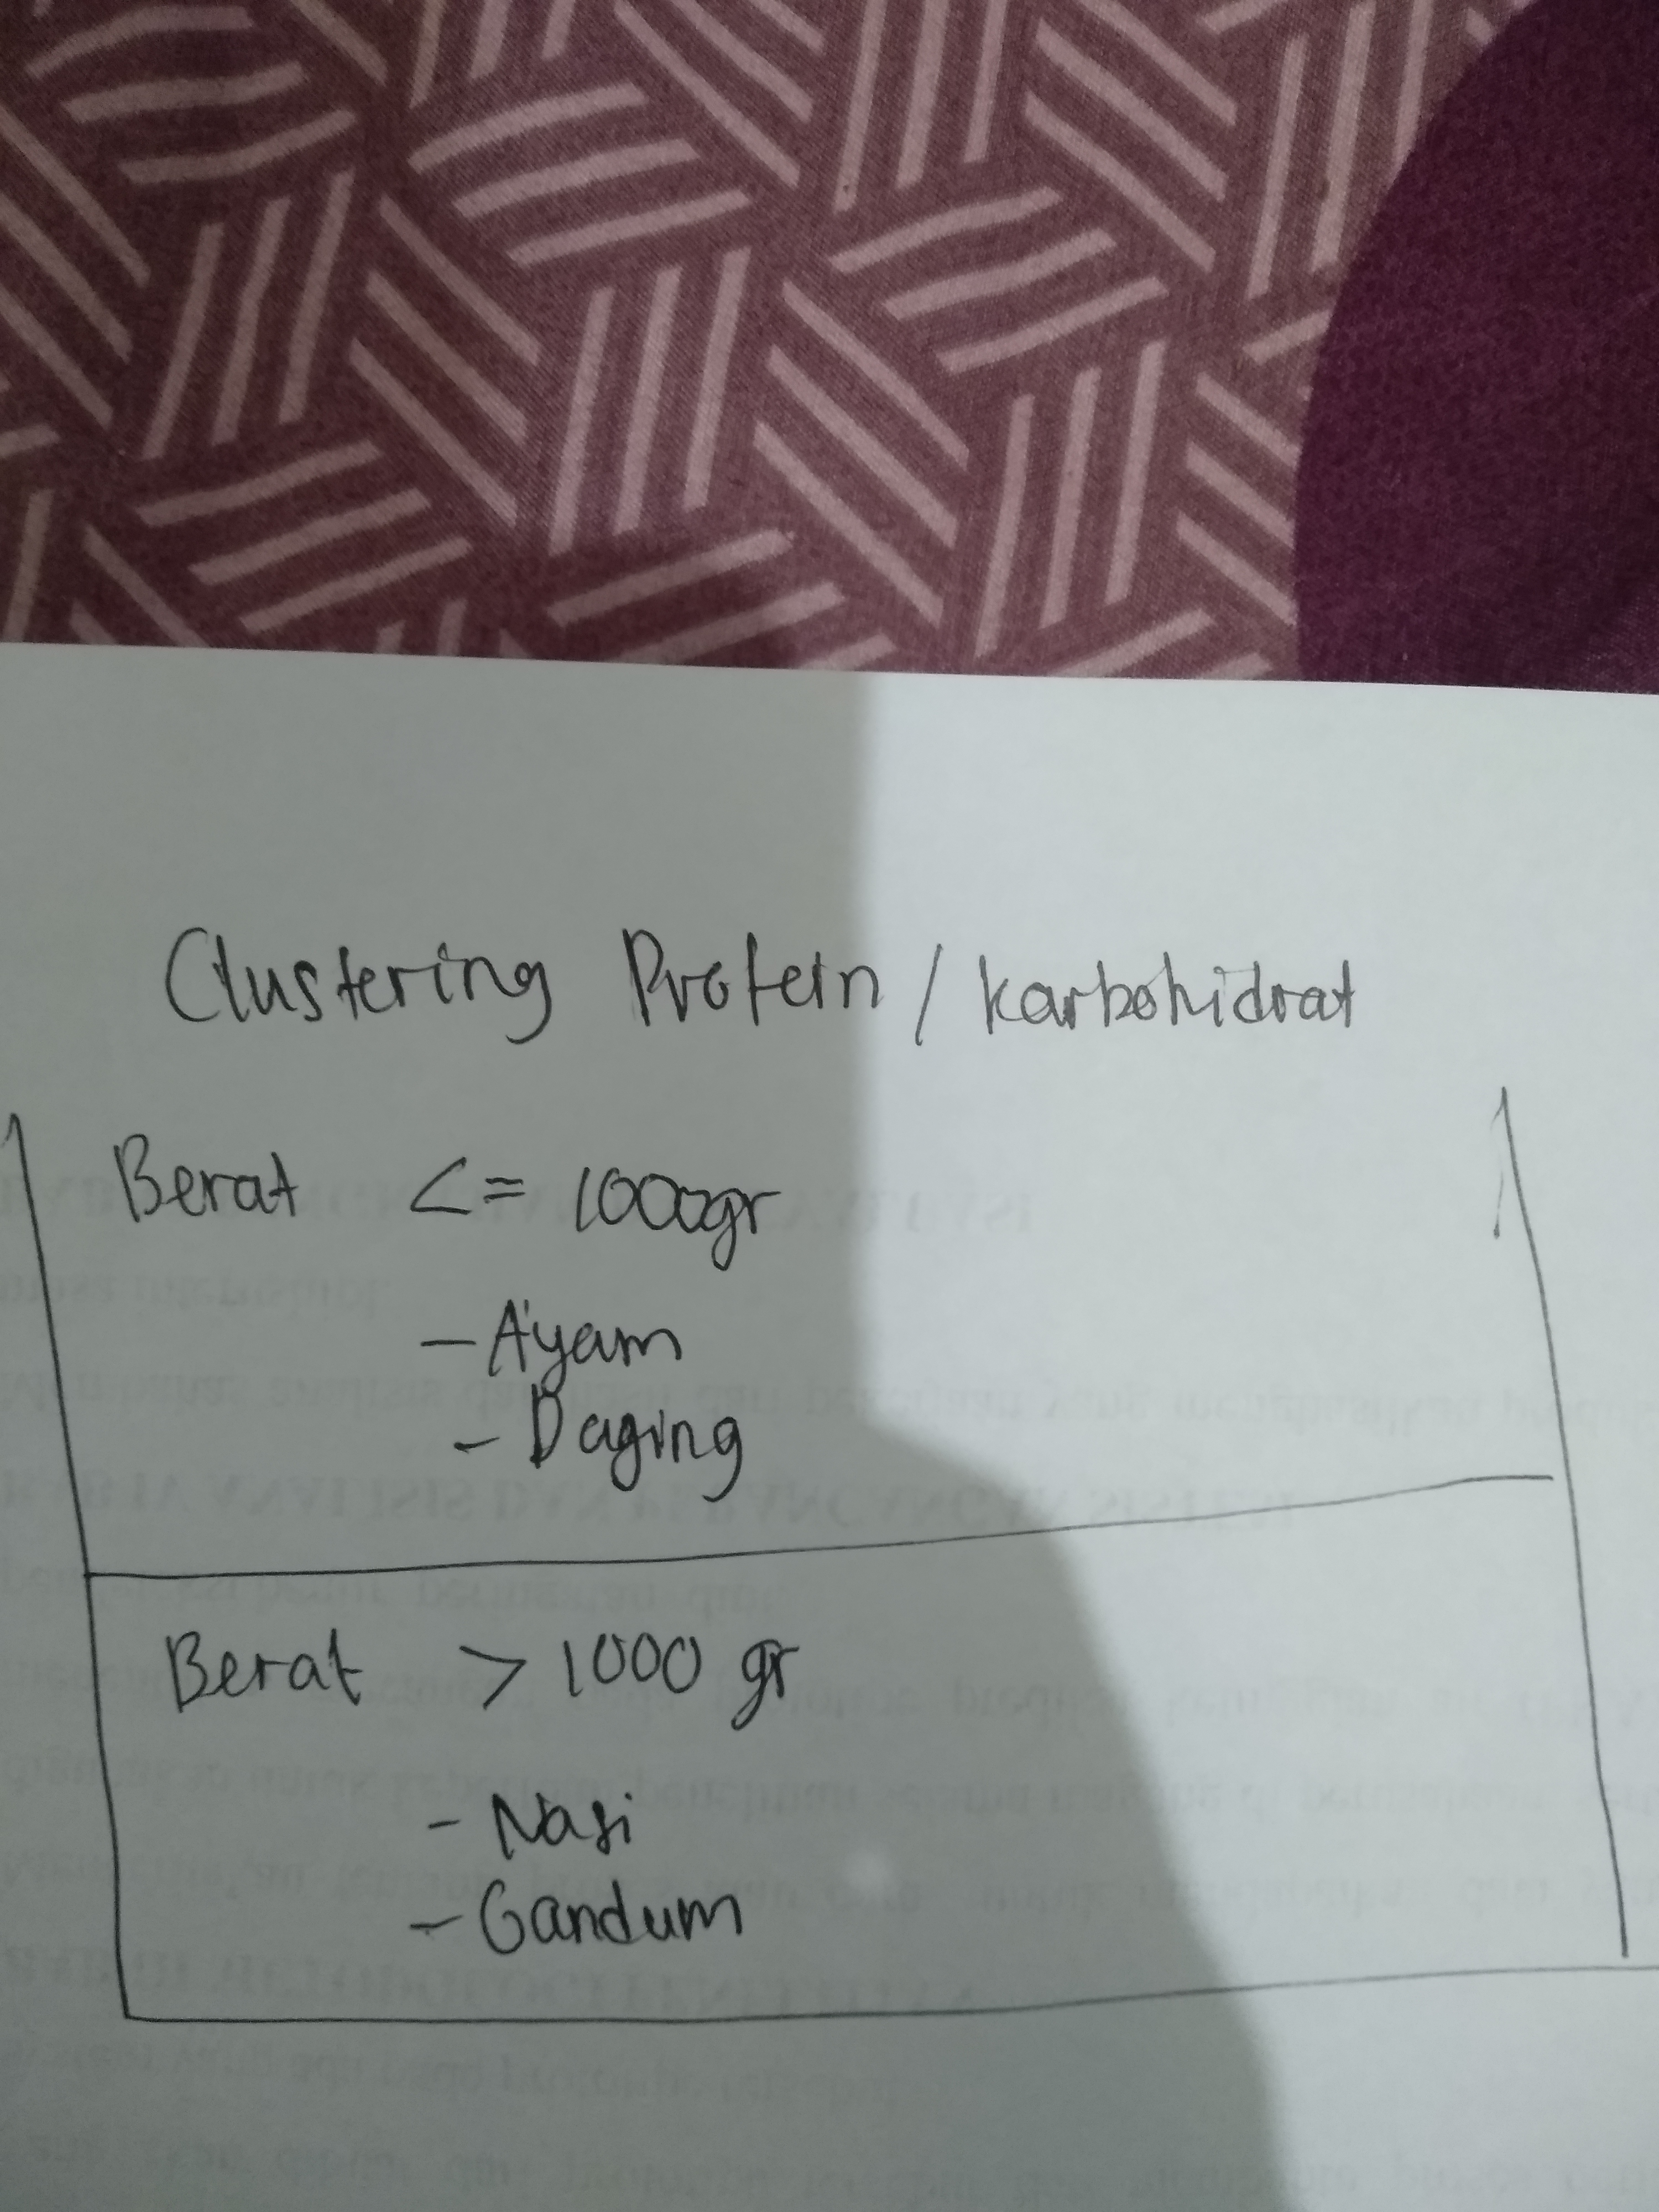
\includegraphics[scale=0.01]{figures/1174050/chapter2/4.jpg}
\caption{contoh clusterring}
\label{contoh}
\end{figure}


\item Jelaskan apa itu evaluasi dan akurasi dan disertai ilustrasi contoh dengan gambar sendiri.\par
evaluasi adalah pengumpulan pengumpulan dan pengamatan dari berbagai macam bukti untuk mengukur dampak efektifitas dari suatu objek, program, atau proses berkaitan  dengan spesifikasi atau persyaratan yang telah di tetapkan sebelumnya. sedangkan akurasi itu sndiri merupakan bagian dari evaluasi yang merupakan ketepatan data terhadap suatu objek berdasarkan keriteria tertentu. kita dappat mengevalluasi seberappa baik modell bekerja denggan menggukur akurasiinya. ketepatan akan di definisikan sebagai presentase kasus yang di klasifikasikan dengan benar. hal ini berkaitan dengan confusion matrix pada materi selanjutnya. contoh evaluasi untuk membedakan angsa dengan entok terdapat parameter yaitu panjang leher dan fungsi sifat dari hewan tersebut. lebih jelanya pada gambar berikut:
\begin{figure}[ht]
\centering
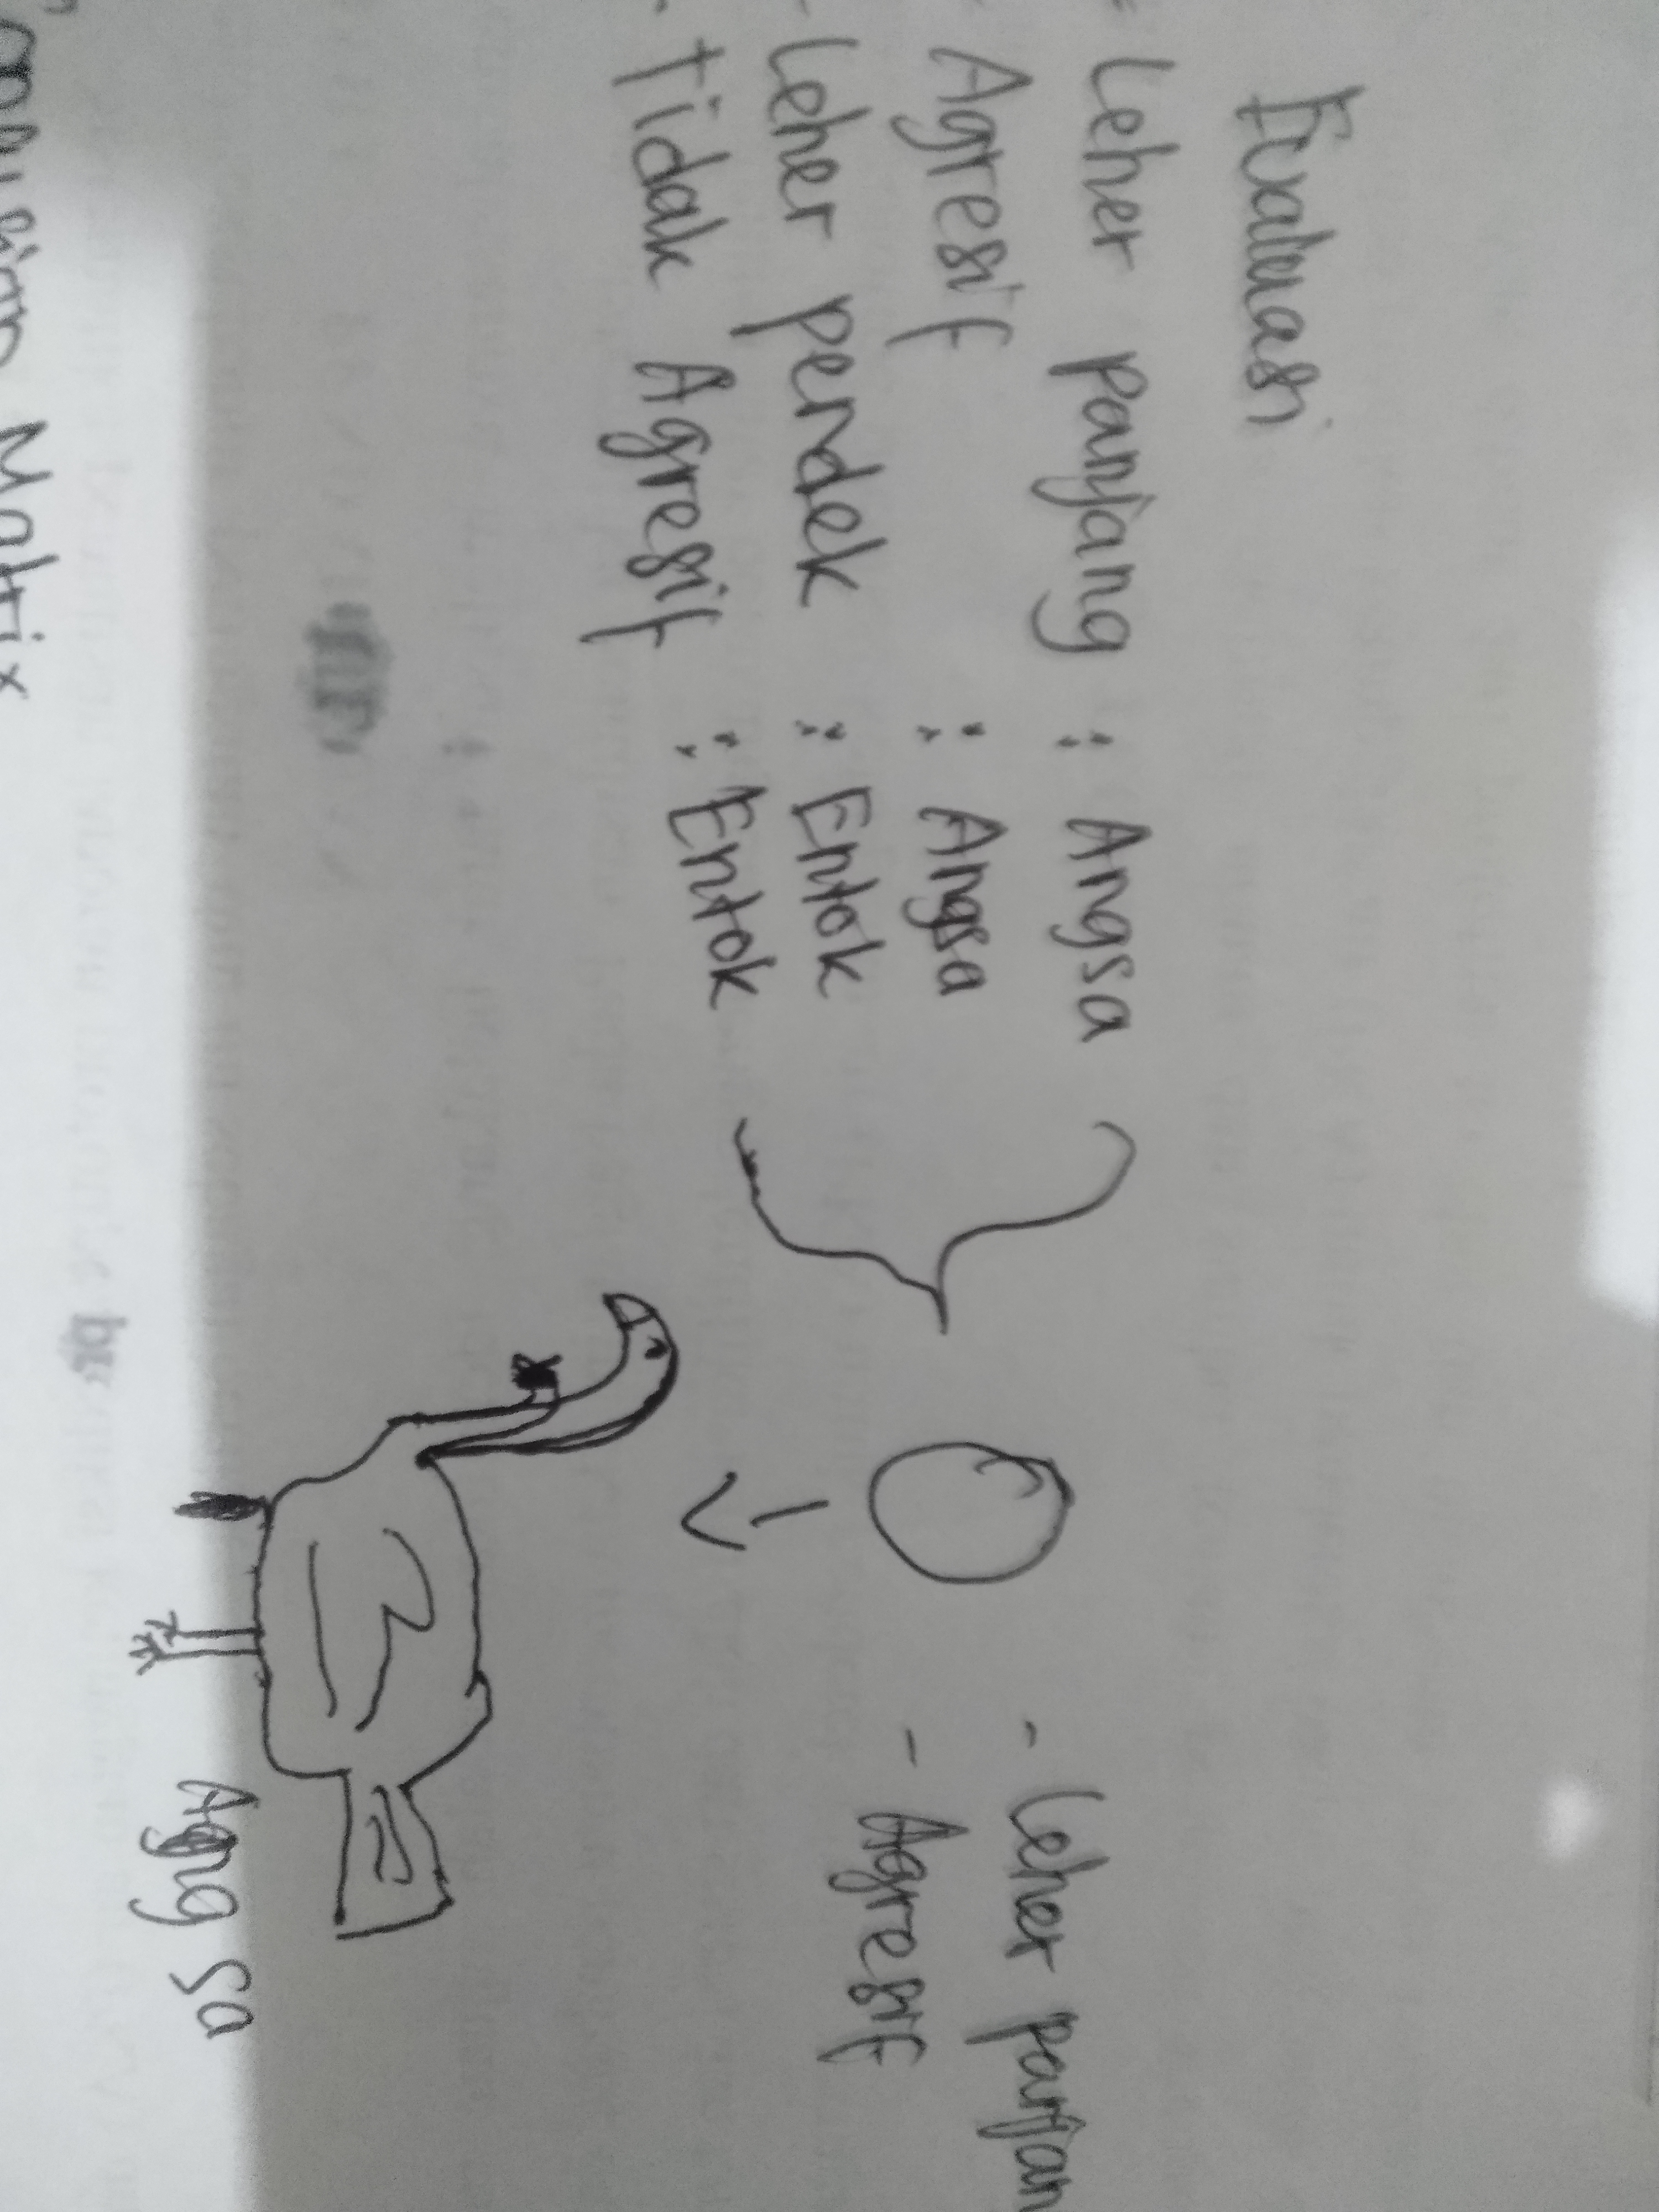
\includegraphics[scale=0.01]{figures/1174050/chapter2/5.jpg}
\caption{contoh evaluasi dan akurasi}
\label{contoh}
\end{figure}


\item Jelaskan bagaimana cara membuat Confusion Matrix, Buat confusion matrix sendiri.\par
Dalam pembuatan confusion matrix tentukan parameter atau objek yang akan di evaluasi contoh angsa,entok, bebek buat tabel dengan baris dan kolom berjumlah tiga kemudian tentukan nilai miring pada setiap kolom tersebut disini saya memberi nilai 15 dengan ketentuan setiap baris harus berisi nilai 15 nilai tersebut jika terbagi ke kolom lain maka jumlahnya harus bernilai 15 jika tidak berarti data tersebut tidak akurat. untuk lebih jelanya dapat dilihat pada gambar berikut :
\begin{figure}[ht]
\centering
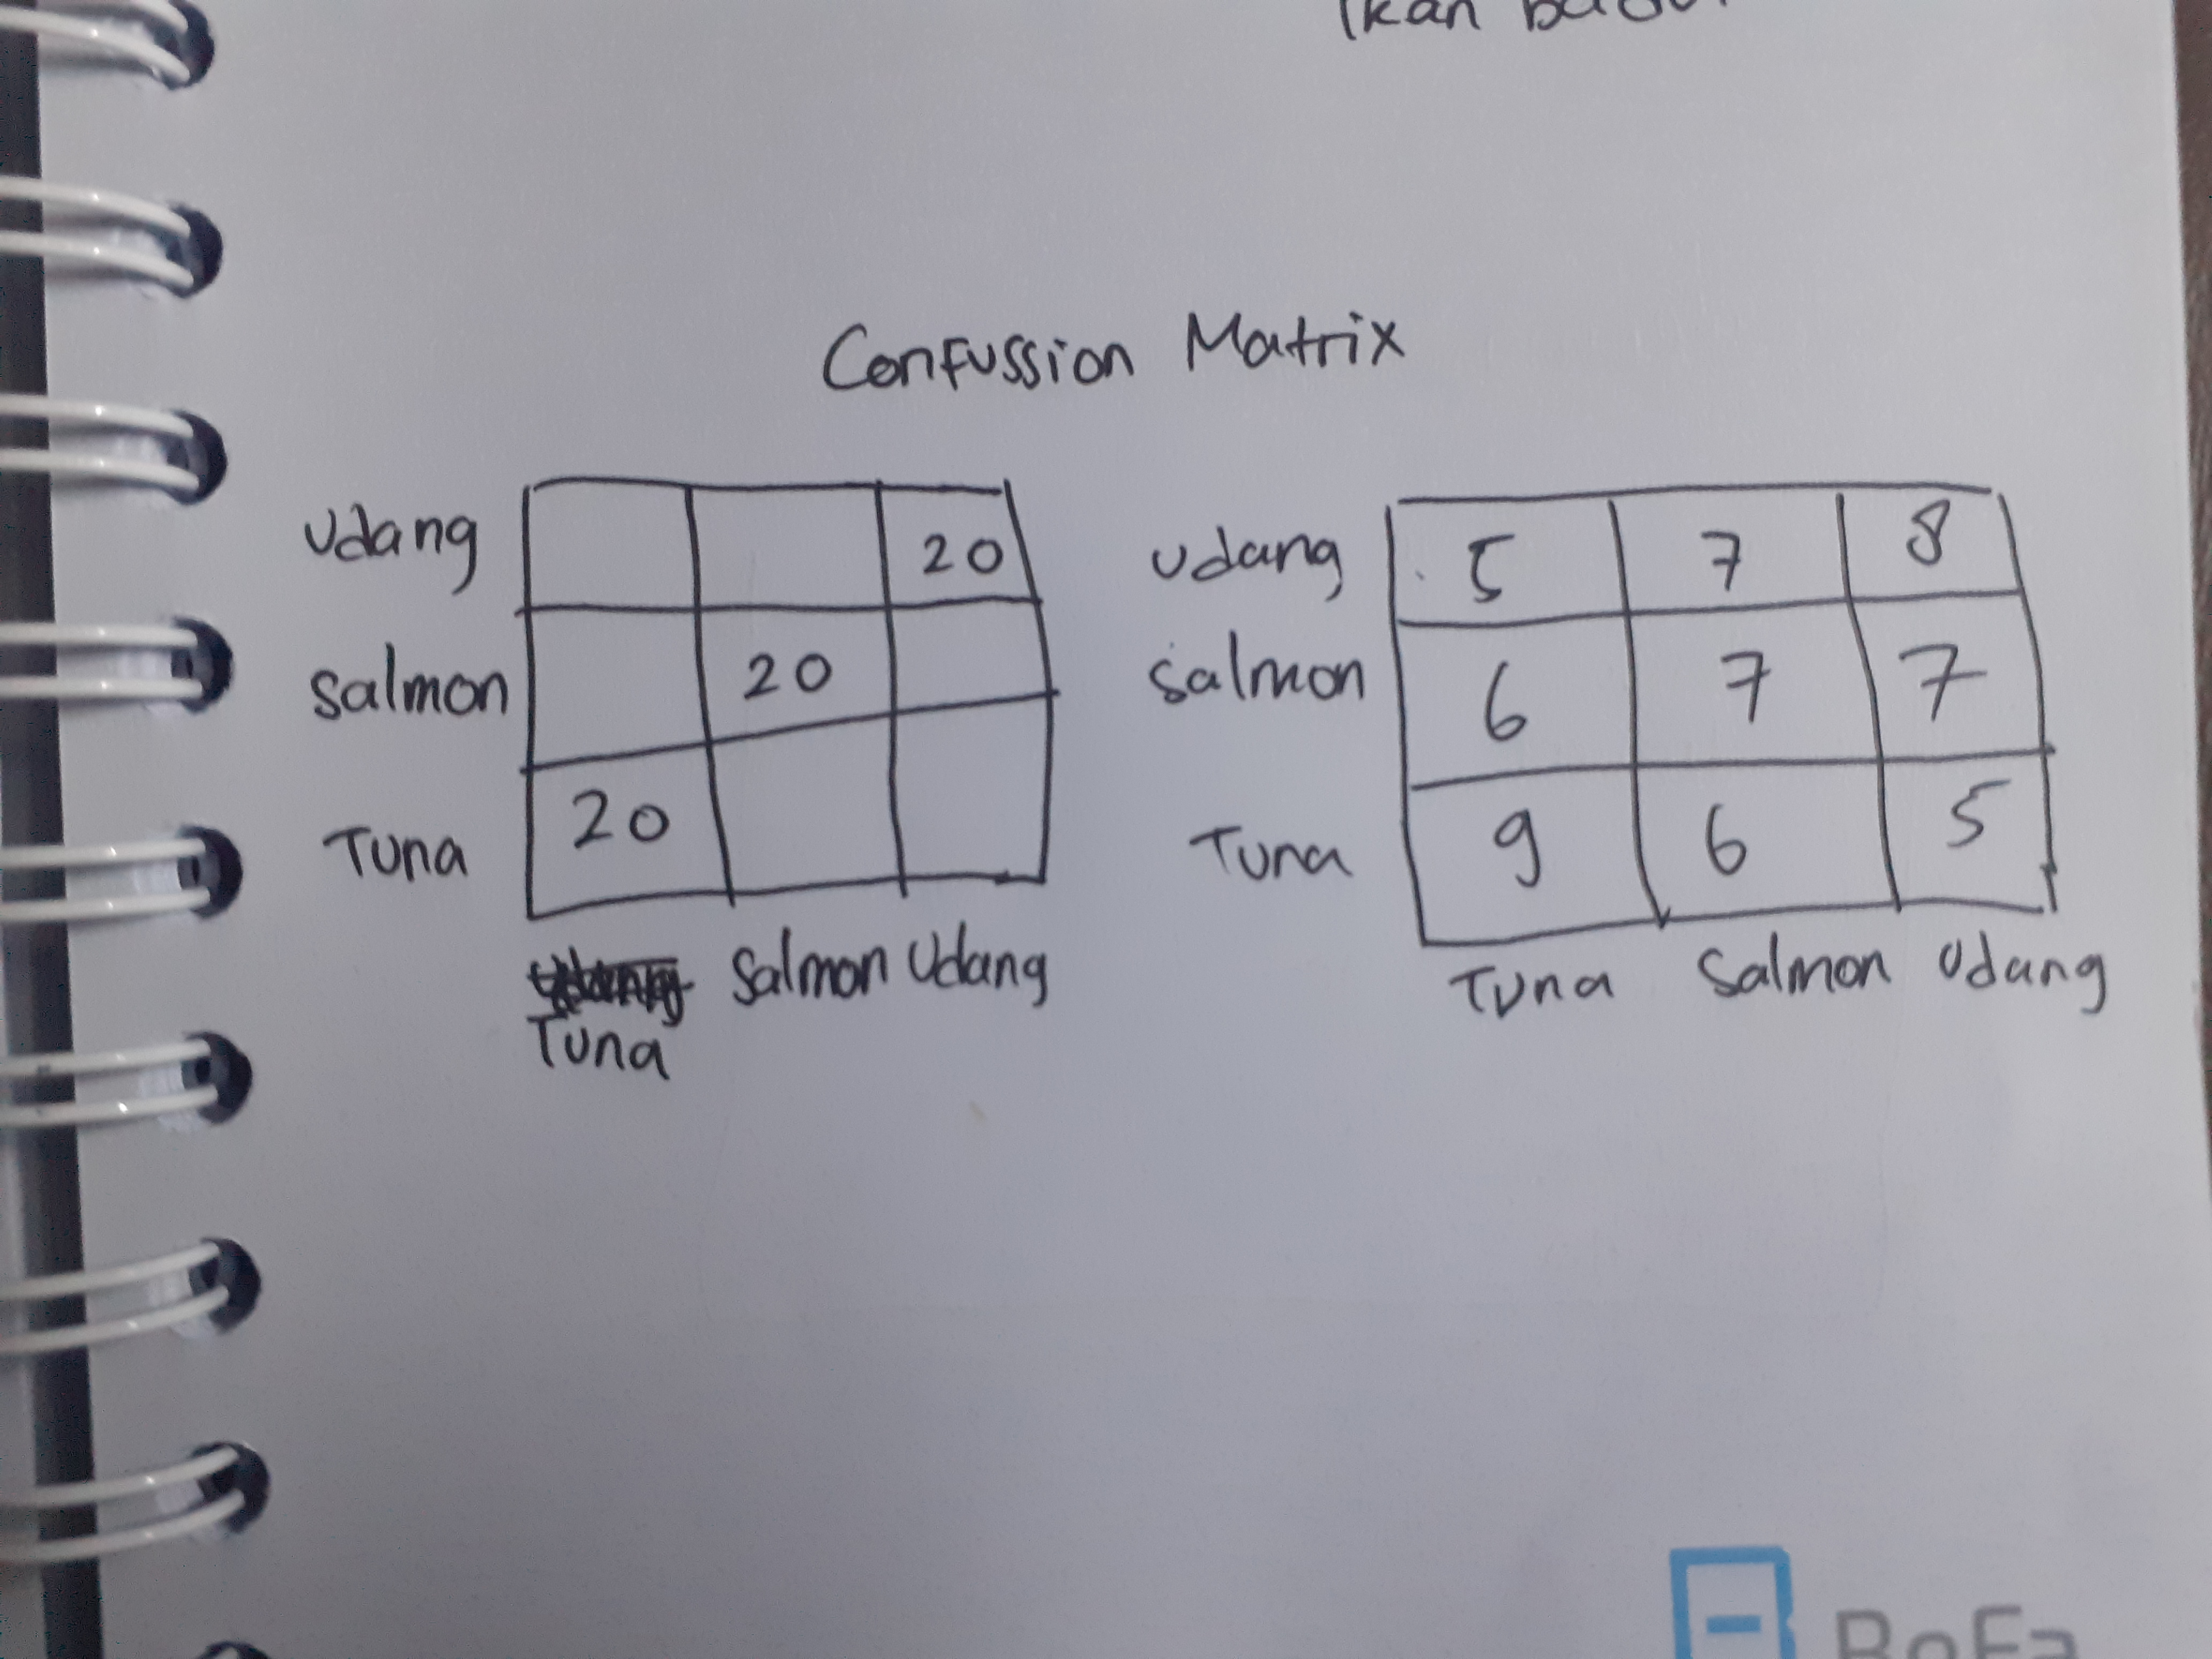
\includegraphics[scale=0.01]{figures/1174050/chapter2/6.jpg}
\caption{contoh Confusion Matrix}
\label{contoh}
\end{figure}


\item Jelaskan bagaimana K-fold cross validation bekerja dengan gambar ilustrasi contoh buatan sendiri.
K-fold Cross Validation merupakan cara untuk melatih suatu mesin dimana di dalammya terdapat data set yang dibagi menjadi dua yaitu untuk data testing dan data training contoh 1000 data merupakan data set dan 300 data digunakan untuk data testing kemudian 700 datanya digunakan untuk data training dimana data training tersebut digunakan untuk menentukan nilai bobot yang dimasukan kedalam rumus regresi linier. sedangkan nilai testing akan dijadikan nili inputan untuk rumus regresi linier. contohnya dapat dilihat pada gambar berikut :
\begin{figure}[ht]
\centering
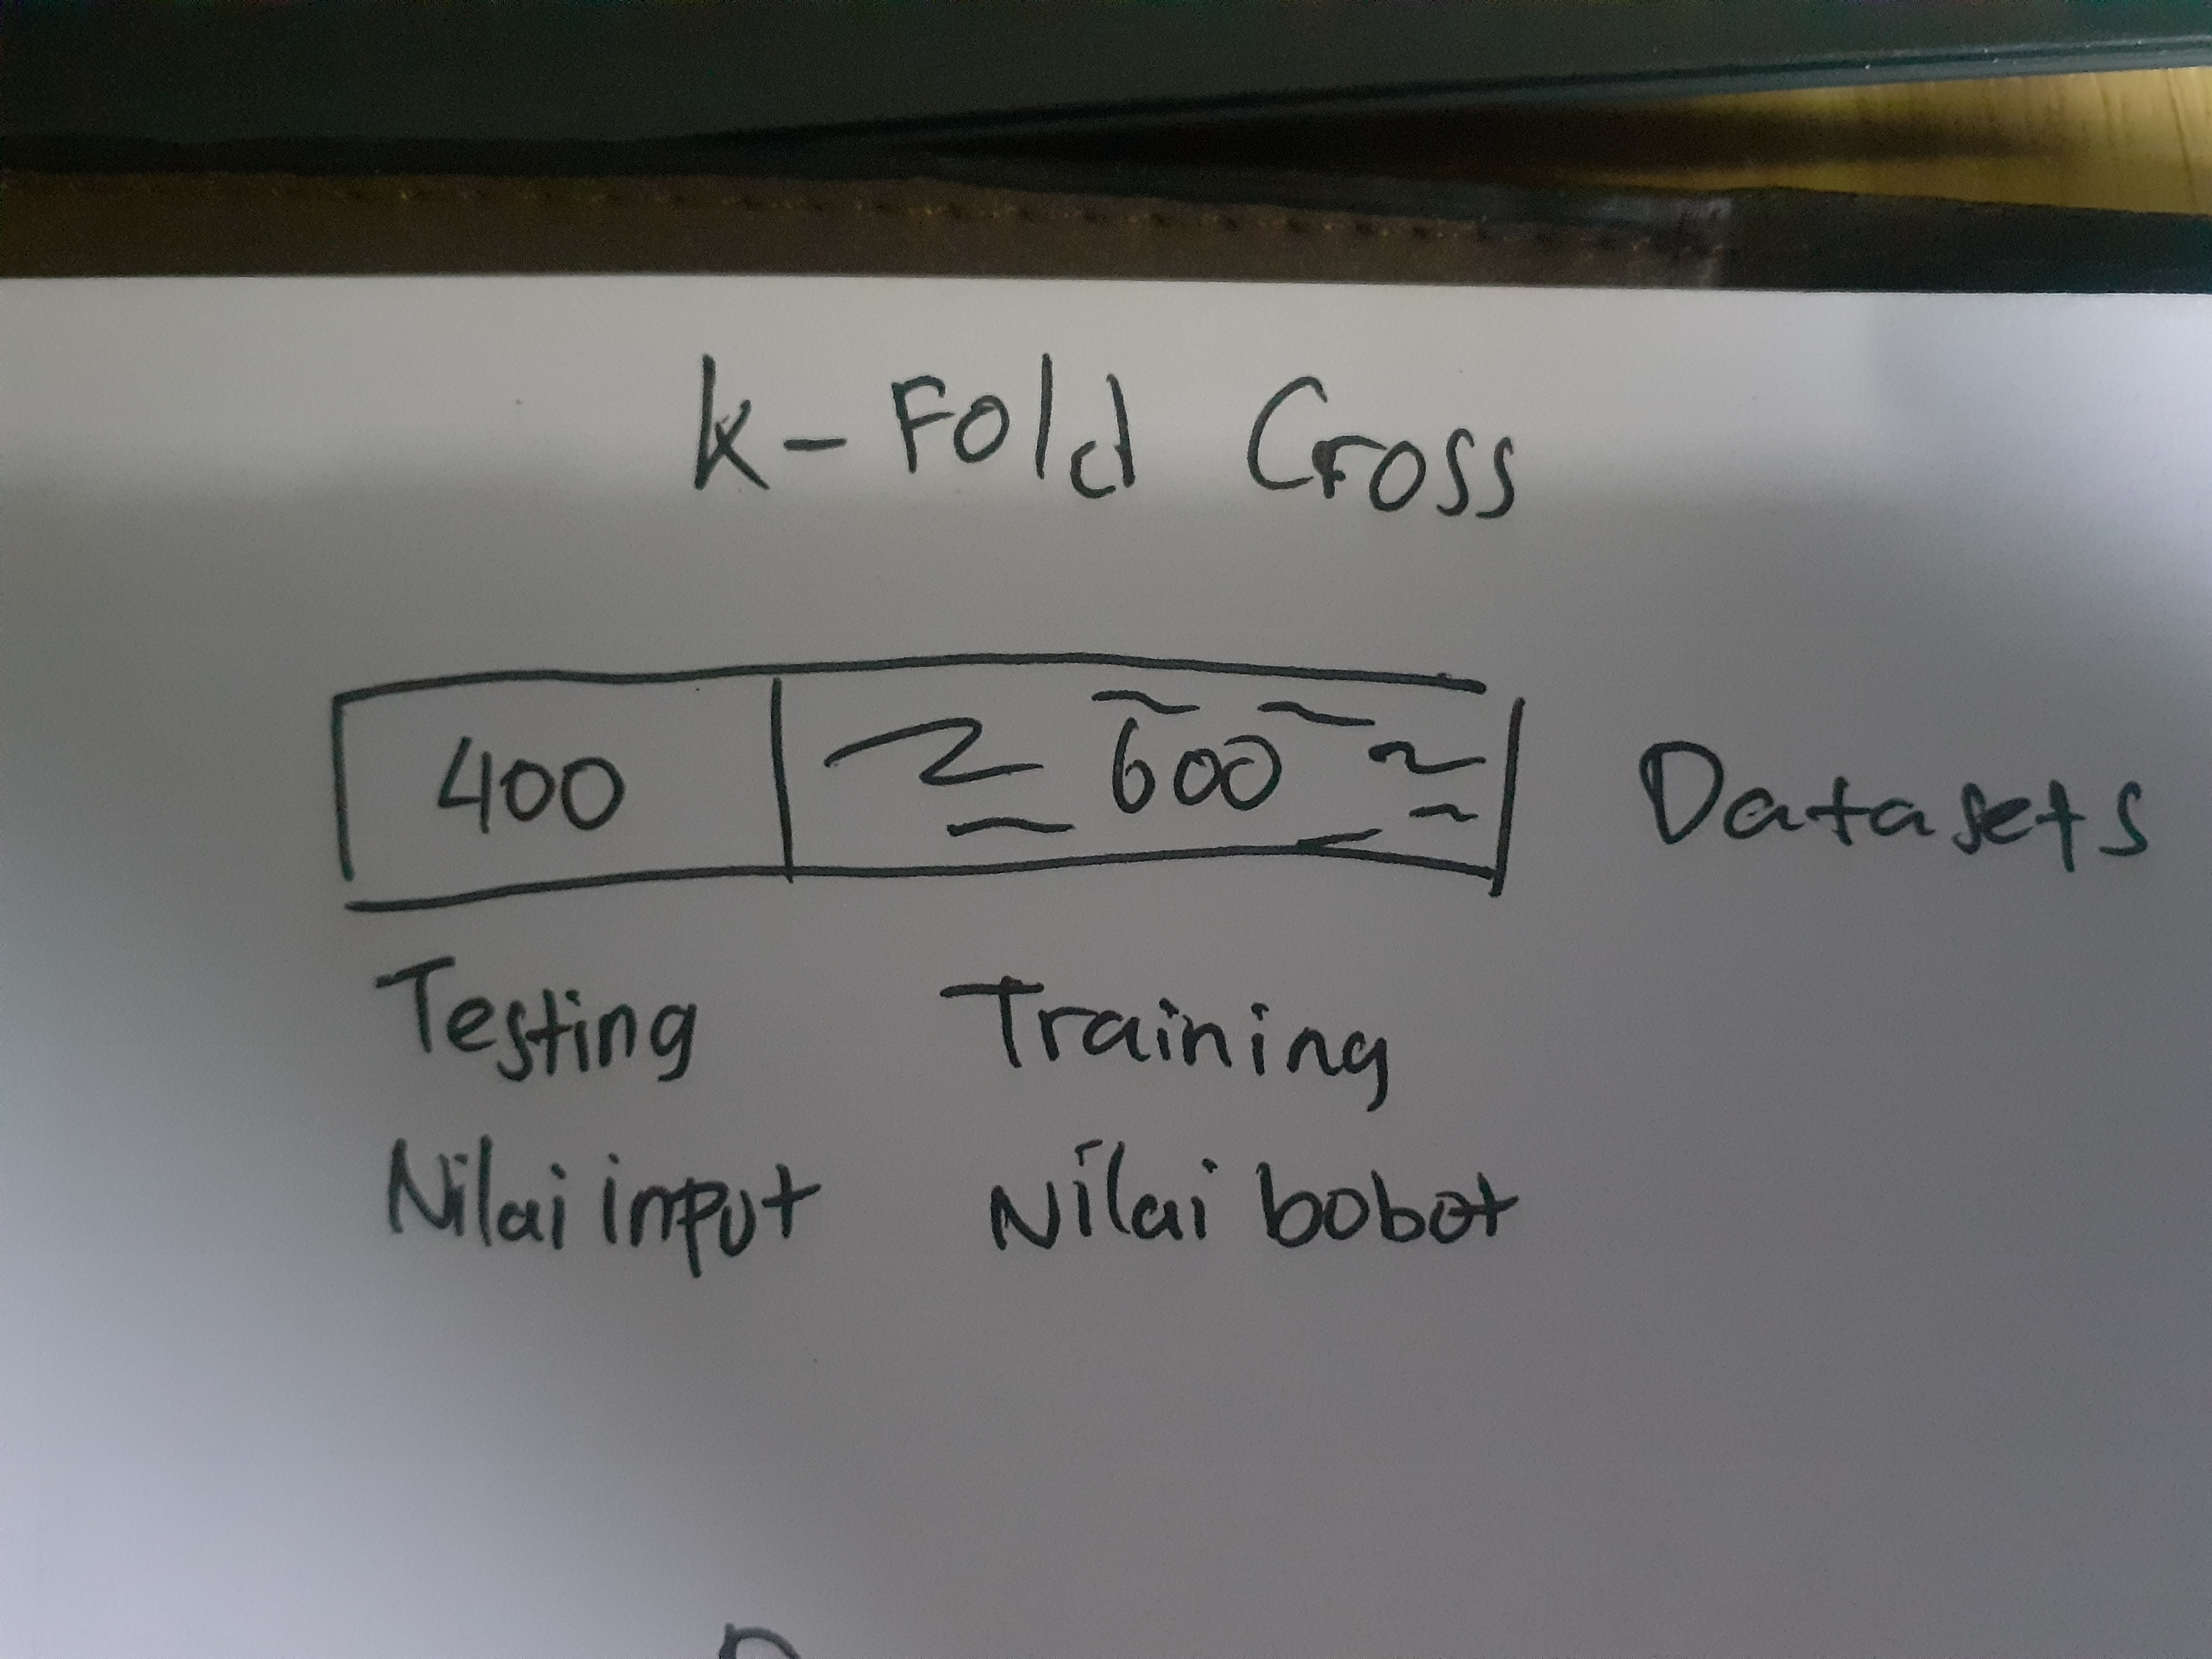
\includegraphics[scale=0.01]{figures/1174050/chapter2/7.jpg}
\caption{contoh K-fold cross validation}
\label{contoh}
\end{figure}


\item Jelaskan Apa itu decision tree dengan gambar ilustrasi contoh buatan sendiri.\par
Decision tree merupakan implementasi dari binari clasification dimana pada pohon keputusan akan terdapat root atau akar dan cabang cabangnya yang nilainya seperti if contoh pada root berisi nilai warna mawar, apakah merah pada cabang satu bernilai iya dan pada cabang dua bernilai tidak jika nilainya iya berarti mawar dan jika tidak maka bukan mawar.
agar lebih jelas dapat dilihat pada gambar decision tree berikut:
\begin{figure}[ht]
\centering
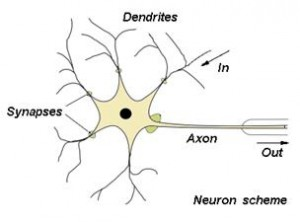
\includegraphics[scale=0.01]{figures/1174050/chapter2/8.jpg}
\caption{contoh decision tree}
\label{contoh}
\end{figure}


\item jelaskan apa itu information gain dan entropi dengan gambar ilustrasi buatan sendiri.\par
informasion gain merupakan informasi atau keriteria dalam pembagian sebuah objek contoh information gain pada llama yaitu leher panjang, ekor panjang, berkaki 4, buas, karnivora. untuk lebih jelasnya dapat dilihat pada gambar berikut :\par
\begin{figure}[ht]
\centering
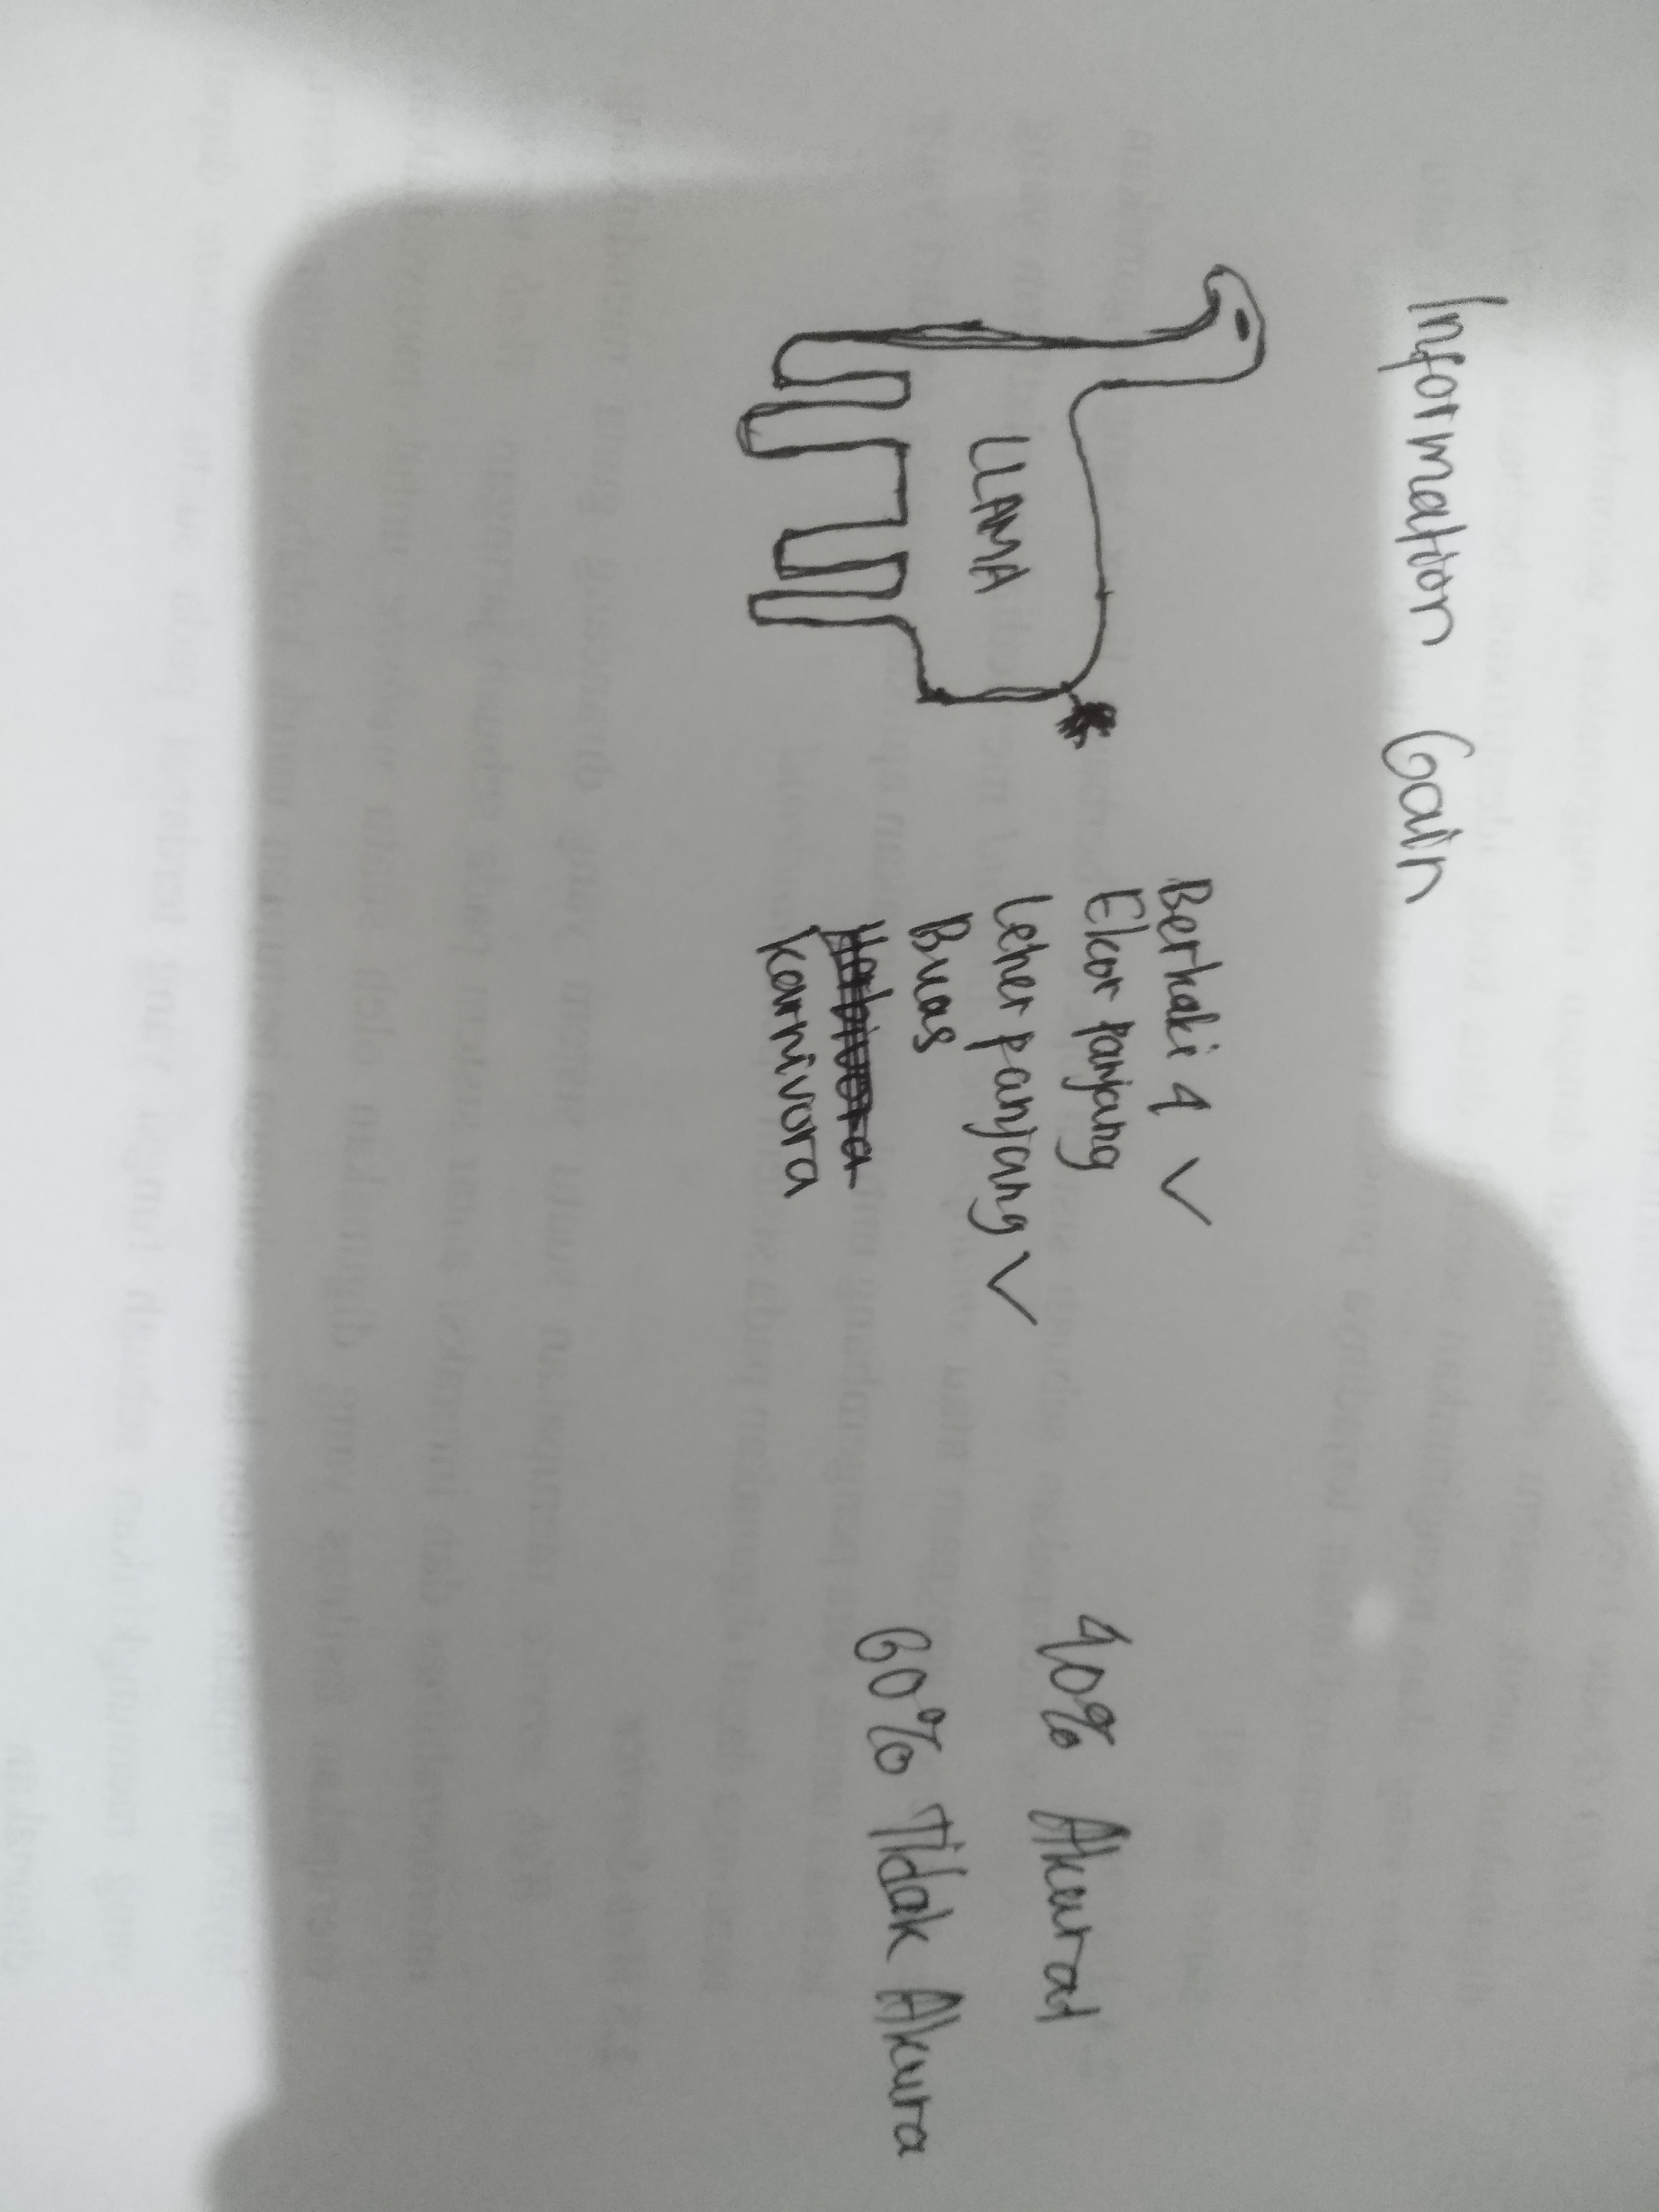
\includegraphics[scale=0.01]{figures/1174050/chapter2/9.jpg}
\caption{contoh information gain}
\label{contoh}
\end{figure}
sedangkan entropi merupakan ukuran keacakan dari informasi semakin tinggi entropi maka semakin sulit dalam menentukan keputusan contoh dalam menentukan satu gen semakin detail informasi maka akan semakin susah dalam menentukan keputusan.
\end{enumerate}







\subsection{Sikic-Learn}
\begin{enumerate}
\item pada surcode pertama yang dapat dilihat pada gambar  pada baris pertama di tuliskan import pandas as baso yang berarti mengimport library padas. selanjutnya pada baris ke dua codingan tersebut berisi code tersebut terdapat variabel pecel yang berisi inisialisasi pandas dengan aksi untuk membaca vfile csv yang terdapat pada direktori pada komputer kemudian terdapat sep samadengan titik koma yang berarti pemisah field di dalam file tersebut merupakan titik koma. kemudian pada bagian akhir terdapat code len (nama variabel) yang berarti akan menghotung jumlah baris pada file tersebut. untuk hasilnya dapat dilihat pada gambar dibawah.
\lstinputlisting{src/1174050/chapter2/1.py}
\begin{figure}[ht]
\centering
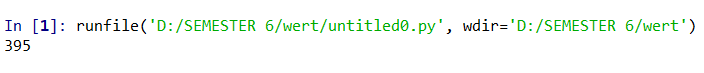
\includegraphics[scale=0.5]{figures/1174050/chapter2/10.PNG}
\caption{hasil}
\label{contoh}
\end{figure}

\item Pada code selanjutnya akan ditambahkan fungsi untuk lulus atau gagal yang dibuat berupa kolom kolom yang di dalammya terdapat nilai 0 dan 1 dimana 0 berarti gagal dan 1 berarti lulus. kemudian variabel pada codingan sebelumnya masih digunakan. dimana variabel pecel digunakan karena berisi nilai file csv kemudian dilakukan ekseskusi dengan parameter G1, G2, dan G3 dengan fungsi lambda yang berarti if bersarang atau if didalam if yang berarti nilai yang di eksekusi akan dilempar ke dalam setiap paramater sasuai dengan kriteria dan axis=1 yaitu nilai tersebut akan digunakan dari tiap baris data. sedangkan pada codingan variabel pecel di berikan aksi drop yaitu penurunan nilai pada bagian baris data. dan pada code pecel.head yaitu untuk mengeksekusi codingan sebelumnya untuk lebih jelasnya dapat dilihat pada gambar dan hasilnya seperti pada gambar berikut :
\lstinputlisting{src/1174050/chapter2/2.py}
\begin{figure}[ht]
\centering
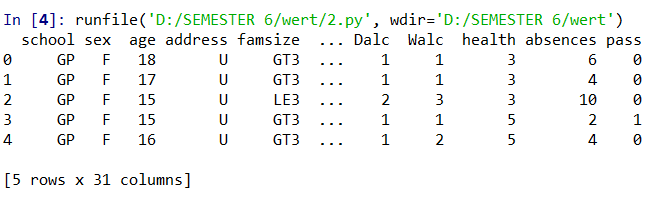
\includegraphics[scale=0.5]{figures/1174050/chapter2/11.PNG}
\caption{hasil}
\label{contoh}
\end{figure}

\item pada kodingan selanjutnya diguanakn untuk menambahkan nilai numerik berupa 0 dan 1 yang dirubah dari nilai tidak dan iya hal ini merupakan fungsi dari codingan get\_dummies pada baris pertama pada gambar yang nilainya diambil dari variabel pecel yang telah di dekralasikan tadi banyaknya data numerik itu sendiri tergantung pada field dari kolom yang di camtumkan pada codingan dengan catatan field tersebut harus ada dalam data csv yang di import oleh codingan pertama tadi maka hasilnya akam merubah data dalam field tersebut menjadi 0 dan 1 untuk lebih jelasnya dapat di lihat pada gambar berikut; 
\lstinputlisting{src/1174050/chapter2/3.py}
\begin{figure}[ht]
\centering
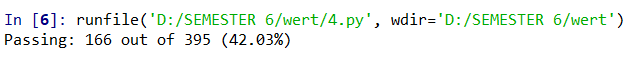
\includegraphics[scale=0.5]{figures/1174050/chapter2/12.PNG}
\caption{hasil}
\label{contoh}
\end{figure}

\item selanjutnya pada codingan selanjutnya yaitu menentukan data training dan data testing dari dataset dimana variabel pecel yang berisi data csv tadi dibuat perbandingan 500 untuk data training dan sisanya yaitu 149 digunakan untuk data testing hal ini di lakukan pada baris ke 1 sampai ke 3 pada gambar kemudian nilai tersebut di turunkan  brdasarkan baris pada data set hal itu dapat dilihat pada baris ke 4 sampai ke 9 pada gambar kemudian selanjutnya mengimport library numpy yang berguna untuk oprasi vektor dan matrix karna data diatas berupa data matrix maka library ini di gunakan. untuk hasilnya dapat dilihat pada gambar.
\lstinputlisting{src/1174050/chapter2/4.py}
\begin{figure}[ht]
\centering
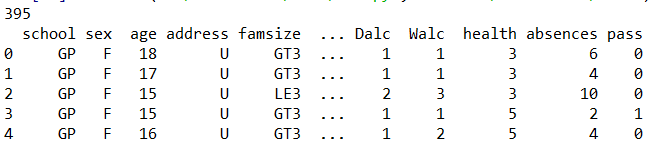
\includegraphics[scale=0.5]{figures/1174050/chapter2/13.PNG}
\caption{hasil}
\label{contoh}
\end{figure}

\item selanjutnya yaitu membuat pohon keputusan dapat lebih jelasnya dapat di lihat pada gambar. pada baris pertama yairu memasukan librari tree kemudian pada baris kedua dibuat variabel lontong dengan nilai DecisionTreeClasifier yang merupakan paket atau fungsi dari scikit-learn yang merupakan class yang mampu melakukan multi class. sedangkan max\_depth=5 merupakan untuk penyesuaian data terhadap pohon keputusan itu sndiri. untuk hasilnya dapat dilihat pada gambar
\lstinputlisting{src/1174050/chapter2/5.py}
\begin{figure}[ht]
\centering
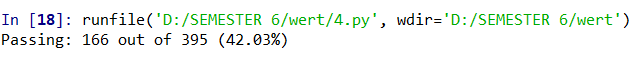
\includegraphics[scale=0.5]{figures/1174050/chapter2/14.PNG}
\caption{hasil}
\label{contoh}
\end{figure}

\item selanjutnya yaitu pembuatan gambar dari pohon keputusan yang tadi di buta pada codingan sebelumnya pada baris pertama codingan ya itu mengimport library graphviz kemudian pada baris ke dua yaitu pemberian nilai pada variabel baru dot data nilainy diambil dari pembuatan puhon keputusan tadi kemudian di tentukannya nilai benar dan salah dari codingan tersebut setelah itu dibuatlah sebuah variabel untuk menampung hasil eksekusi tersebut kemudian variabel tersebut di running untuk lebih jelasnya dapat di lihat pada gambar.kemudian hasilnya dapat dilihat pada gambar.
\lstinputlisting{src/1174050/chapter2/6.py}
\begin{figure}[ht]
\centering
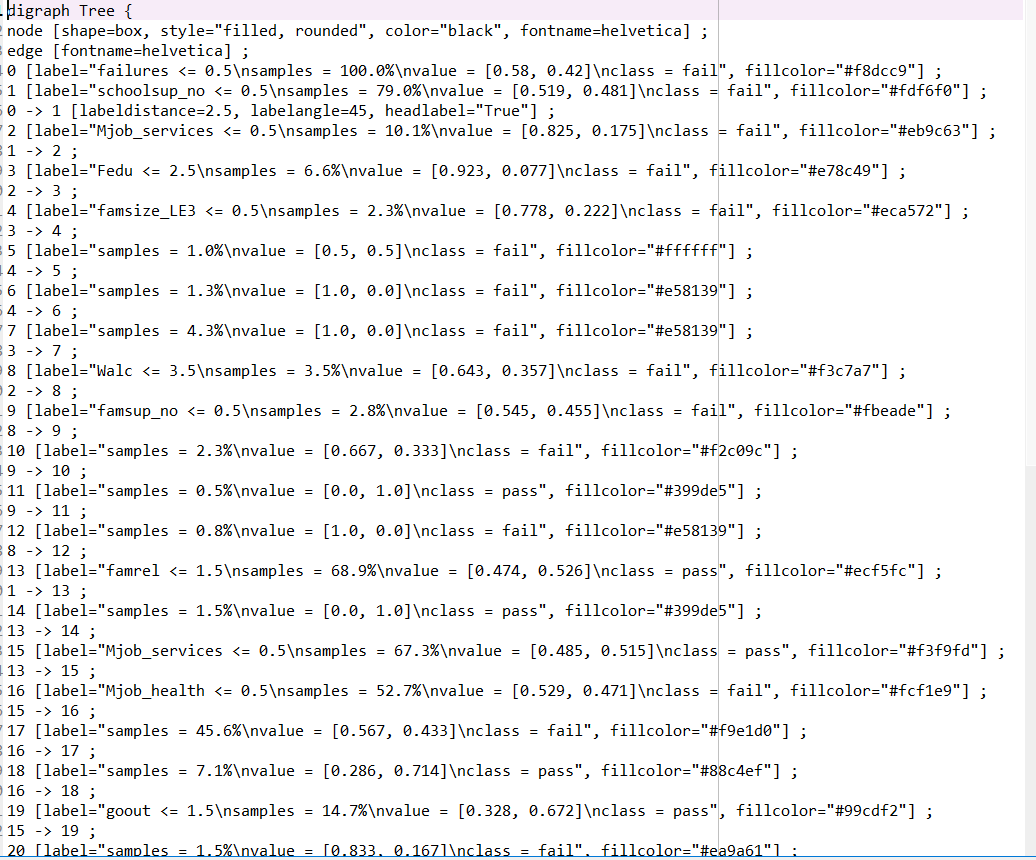
\includegraphics[scale=0.5]{figures/1174050/chapter2/15.PNG}
\caption{hasil}
\label{contoh}
\end{figure}

\item selanjutnya pembuatasn method untuk menyimpan data pohon dengan menarik data langsung dari pohon keputusan di buat tadi untuk code lebih jelasnya dapat dilihat pada gambar. kemudian intuk hasilnya dapat dilihat pada gambar berikut.
\lstinputlisting{src/1174050/chapter2/7.py}
\begin{figure}[ht]
\centering
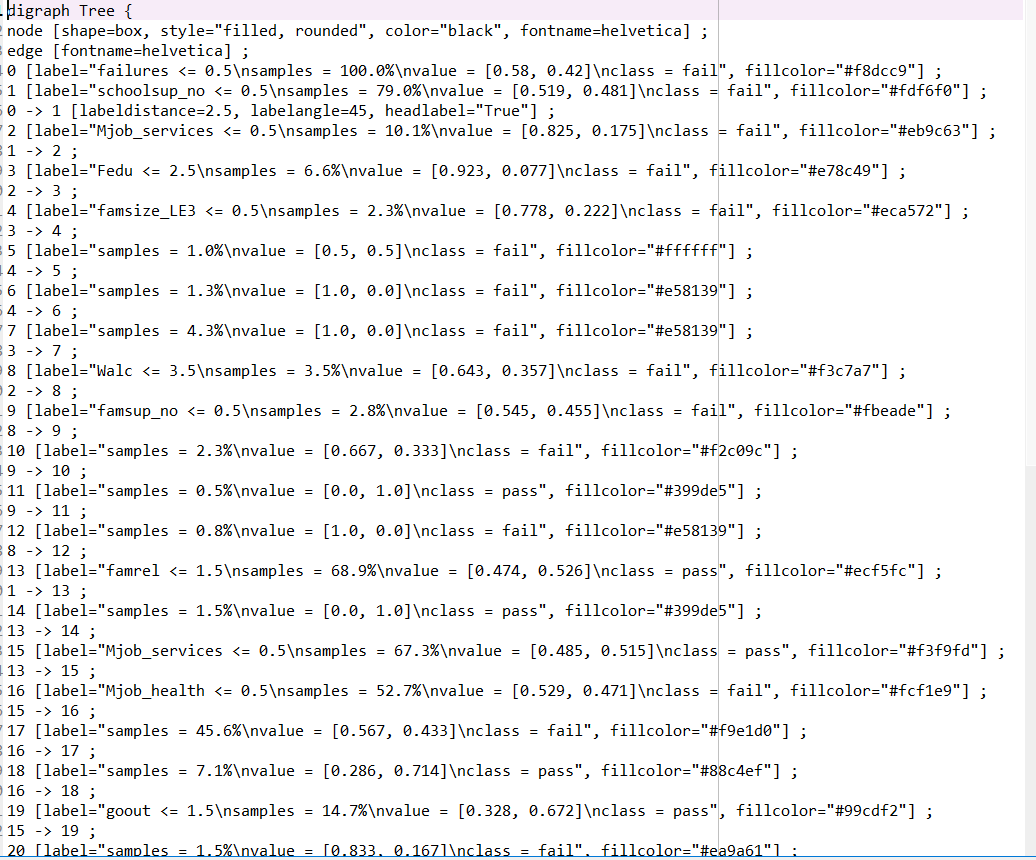
\includegraphics[scale=0.5]{figures/1174050/chapter2/15.PNG}
\caption{hasil}
\label{contoh}
\end{figure}

\item selanjutnya pada codingan berikut yaitu digunakan untuk mencetak nilai score rata-rata dari ketepatan data yang telah di olah tadi lebih jelsnya dapat dilihat pada gambar kemudian untuk hasilnya dapat dilihat pada gambar tersebut:
\lstinputlisting{src/1174050/chapter2/8.py}

\item selanjutnya yaitu digunakan untuk memeriksa akurasi dari ketepatan hasil pengolahan data tersebut maka akan didapat nilai rata-rata 60 persen dari hasil pengolahan data tersebut untuk lebih jelasnya dapat di lihat pada gambar pada codingan tersebut pada baris ke satu melakukan import library dari sklern kemudian pada baris selanjutnya mengisi nilai skor dengan nilai pada variabel lontong setelah hal tersebut dilakukan kemudian data tersebut di eksekusi. berikut merupakan hasil dari code tersebut dapat dilihat pada gambar.
\lstinputlisting{src/1174050/chapter2/9.py}
\begin{figure}[ht]
\centering
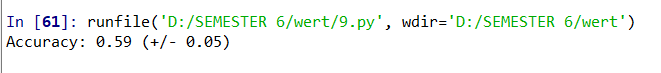
\includegraphics[scale=0.5]{figures/1174050/chapter2/16.PNG}
\caption{hasil}
\label{contoh}
\end{figure}

\item membuat rank akurasi dari 1 sampai 20 untuk melihat akurasi data apakah datatersebut terdapat di rata rata 60 persen atau tidak dengan cara membuat lagi variabel baru dengan nilai tree diadalammya jadi hampir mirip seperti membuat pohon keputusan namun ini langsung dalam bentuk rata rata akurasi yanlebih spesifik untuk lebih jelasnya dpat dilihat pada gambar codingan berikut. dan untuk hasilnya dapat dilihat pada gambar berikut.
\lstinputlisting{src/1174050/chapter2/10.py}
\begin{figure}[ht]
\centering
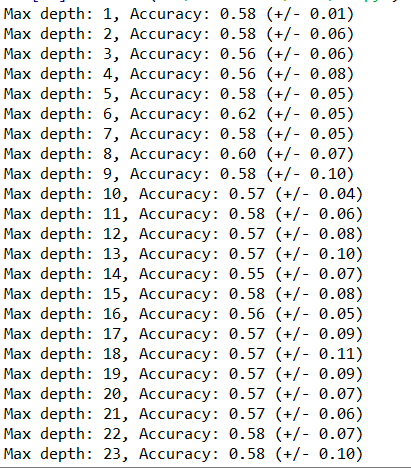
\includegraphics[scale=0.5]{figures/1174050/chapter2/19.PNG}
\caption{hasil}
\label{contoh}
\end{figure}

\item untuk selanjutnya yaitu menentukan nilai untuk grafik hampirsama dengan nilia akurasi tadi pertama tentukan rank atai batasan nilai itu disini batasannya di mulai dari 1 sampai 20 dengan menggunakan nilai tree tadi maka hasilnya dapat ditentuka kemudian buat variabel i untuk penomoran tiap record yang keluar atau recod hadil dari eksekusi tree tersebut. untuk lebih jelasnya dapat dilihat pada gambar dan untuk hasilnya dapat dilihat pada gambar.
\lstinputlisting{src/1174050/chapter2/11.py}
\begin{figure}[ht]
\centering
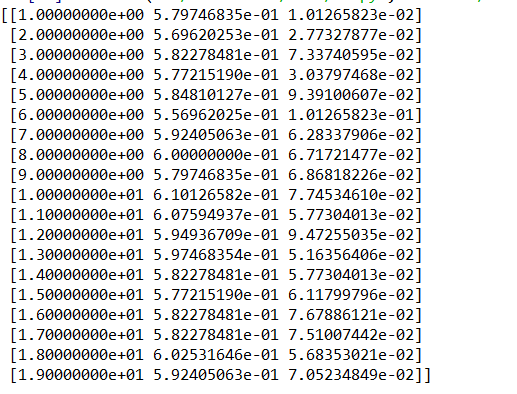
\includegraphics[scale=0.5]{figures/1174050/chapter2/17.PNG}
\caption{hasil}
\label{contoh}
\end{figure}

\item terakhir yaitu pembuatan grafik untuk pembuatan grafik diambil data dari codingan sebelumnya yang 20 record tadi dengan cara mengimport libray matplotlib.pyplot yang di inisialisasi menjadi bakwankemudian inisialisasi tersebut di eksekusi. untuk lebih jelasnya codingannya seperti gambar dan untuk hasilnya seperti gambar  berikut. 
\lstinputlisting{src/1174050/chapter2/12.py}
\begin{figure}[ht]
\centering
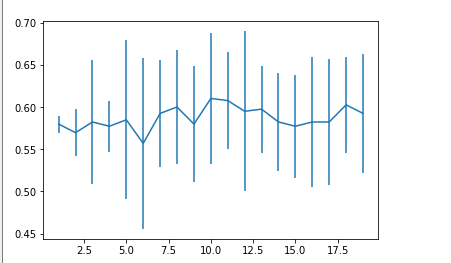
\includegraphics[scale=0.5]{figures/1174050/chapter2/18.PNG}
\caption{hasil}
\label{contoh}
\end{figure}
\end{enumerate}

\subsection{Penanganan Error}
\begin{enumerate}
\item skrinsut error
\begin{figure}[ht]
\centering
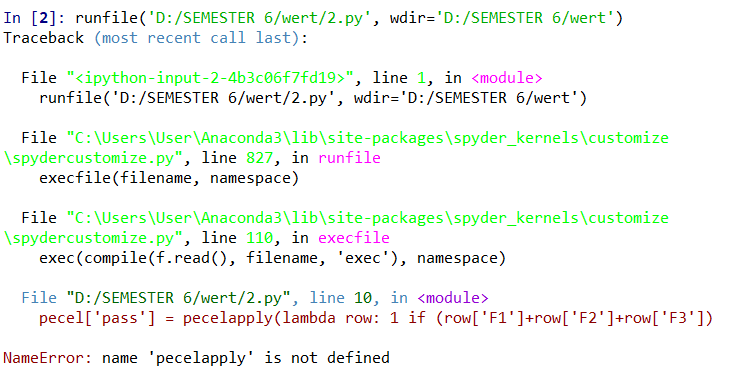
\includegraphics[scale=0.5]{figures/1174050/chapter2/error.PNG}
\caption{Error}
\label{contoh}
\end{figure}

\item kode error dan jenis errornya .
\begin{verbatim}
pecel['pass'] = pecelapply(lambda row: 1 if (row['G1']+row['G2']+row['G3'])
>= 35 else 0, axis=1)
pecel = pecel.drop(['G1', 'G2', 'G3'], axis=1)
print(pecel.head())
\end{verbatim}

NameError: name pecelapply is not defined

\item Solusi pemecahan masalah \par
pada codingan tersebut error karena pecelapply tergabung, seharusnya dipisahkan oleh titik
\end{enumerate}


\subsection{Plagiat}
\begin{figure}[ht]
\centering
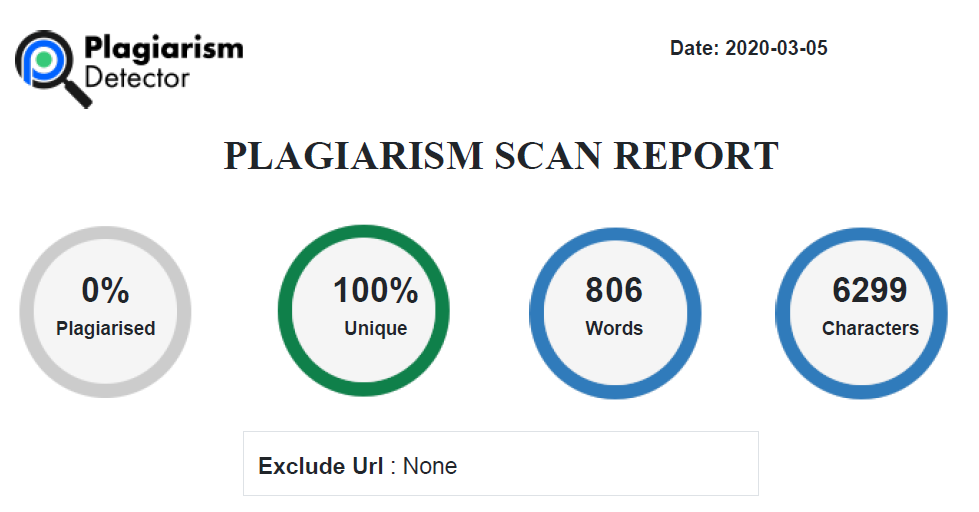
\includegraphics[scale=0.5]{figures/1174050/chapter2/plagiarism.PNG}
\caption{Error}
\label{contoh}
\end{figure}
